\chapter{Precursor Clustering of Ionisation Product Peaks}
\label{c:precursor-clustering}

\section{Introduction}

\textbf{It reads very well. If I were an examiner and I read this, I’d be happy — i.e., all my comments are pretty minor — well done!
I think you could make a bit more of the adduct fingerprint. It’s not mentioned in the intro. As I see it, one benefit of the cluster-cluster method is that it offers a principled approach to incorporating additional information (through adding likelihood terms). In this context, the adducts are an example rather than an end in themselves.
I couldn’t see any evidence of statistical testing in the results, although the word ‘significant’ appears in the text. As you’re averaging over datasets, it should be possible to do some tests? If not, then avoid loaded words like ‘significant’.
The conclusions are like a paper’s conclusions (no surprises there). You have no space limitations here, so it would be good to broaden them if possible. e.g. where could this lead (HDP?) etc}

Chapter~\ref{c:matching} explores the idea of using the grouping of related peaks to modify the similarity scores used for matching with the aim of improving alignment results. However, the grouping of related peaks used by the MWG and MWM methods in Chapter~\ref{c:matching} is performed based on the retention time alone. Valuable information present in the mass domain and also in the chemical relationships of related peaks is not used in the grouping process. In this work, we extend upon the methods in the previous chapter and propose a novel Bayesian mixture model (PrecursorCluster) to perform the ionization product clustering of related peak features based on mass, retention time and a list of possible ionization transformations --- bringing together peaks that share chemically meaningful relationships and can be related to a common precursor mass according to a set of transformation rules configurable by the user. 

Building upon the results returned by PrecursorCluster, two alternative alignment methods (illustrated in Figure~\ref{fig:01}) are introduced for aligning IP clusters across runs: \textbf{(i)} Cluster-Match, a fast direct-matching method of IP clusters that uses the posterior precursor mass and RT values of IP clusters to compute the approximate maximum-weighted matching of the IP clusters and \textbf{(ii)} Cluster-Cluster, a second-stage clustering model that constructs alignment by means of grouping the IP clusters according to their likelihood of being assigned to the same same top-level cluster (in this manner, IP clusters assigned to the same top-level cluster are considered to be matched). 

The aim of this chapter is to evaluate whether through the proposed methods, the matching of IP clusters can improve upon the matching of LC-MS peak features alone. For the purpose of evaluations, two benchmark datasets of standard and beer mixtures, alongside their associated alignment ground truth and a list of 14 adduct transformations in positive ionization mode, were used. Using precision, recall and $F_1$-score as evaluation measures, the performance of the proposed method of matching IP clusters (Cluster-Match) were compared against the direct matching of peak features (MW) and its variant (MWG) that modifies the similarity matrix used during matching to bring together group of peaks related by RT closer during matching (described in Chapter~\ref{c:matching}). Additionally, the probabilistic matching results produced by Cluster-Cluster is also described, demonstrating that it is possible to use its output to extract aligned peaksets with varying degrees of confidence.

\section{Related Work}

According to \cite{Smith2015}, the alignment objective function can be improved by operating on the groupings of related IP peaks rather than at the individual peak level alone. In MetAssign \cite{Daly2014}, a Bayesian mixture model was introduced to perform the identification of a set of observed peaks based on how well they fit the theoretical mass spectrum of a metabolite computed from a given formula. While the groupings of related peaks extracted from PrecursorCluster naturally lend themselves to interpretation and can potentially be used in a similar manner as MetAssign, to perform a more robust annotation of metabolites present the sample, here we investigate its uses in improving the alignment step. Unlike MetAssign, PrecursorCluster does not require a prior library of possible metabolite formulas to be specified to perform ionization product clustering, relying only on prior chemical knowledge of which ionization transformations are expected to be present in the data. Unlike CAMERA \cite{Kuhl2012}, which approaches the problem of ion species annotation from a graph-theoretic point-of-view, PrecursorCluster is a fully probabilistic model, relying on Bayesian inference to update the probabilities of which LC-MS peak features can be explained by which transformations into IP clusters. This additional information can be used to provide an estimate to the uncertainty of IP annotations. The Bayesian model proposed in PrecursorCluster can also be easily extended to incorporate additional sources of information (e.g. chromatographic peak shapes) for clustering peaks in a different manner. 

Since alignment is such an important part of the data preprocessing steps, it is useful to be able to robustly identify the uncertainty or confidence in the alignment results. In the absence of ground truth information (typically the case in untargeted metabolomics experiment), the user measures alignment quality through manual inspection or by comparing and visualising the summary statistics (e.g. median, standard deviation of retention time) across different replicates. Alignment methods that can produce matching confidence values is a big research gap that, to our knowledge, has not been addressed by any of existing direct-matching tools. Tools such as MAVEN \cite{Melamud2010} assigns quality scores to individual peaks by training a predictive model on expert-annotated training data of peak quality metrics, but this does not extend to scoring groups of peaks. Other approach like \cite{Brodsky2010} computes the Pearson correlations between intensity profiles of all peaks across replicates. Moving from these approaches towards a robust method that can provide confidence values for groups of aligned peaks across many label-free experiments is challenging research problem.

The subject of identifying and quantifying uncertainty has been extensively investigated in the problem of multiple sequence alignment (MSA) for genomics and transcriptomics. \cite{Landan2009} attempt to quantify the alignment uncertainty of the popular MSA tool ClustalW \cite{Thompson1994}, based on evaluations using synthetic data, and concludes that between half to all columns in their benchmark MSA results contain alignment errors. \cite{Notredame2000} construct a score that reflects the consensus between all possible pairwise alignments in T-COFFEE, while \cite{Penn2010} propose GUIDANCE, a confidence measure obtained from pertubations of guide trees. Statistical approaches that provide a measure of confidence in alignment results have also been explored by \cite{Redelings2005} and \cite{Bradley2009}, where the MSA results and phylogeny are constructed simultaneously, thus eliminating the need for a guide tree. 

Despite the clear benefits of alignment uncertainty quantification in the sequence domain, the challenge of quantifying alignment results remains relatively unaddressed for the alignment of multiple runs in LC-MS-based-omics \textbf{You didn't say WHY the probabilities are good?}. Bayesian methods operating on profile data (e.g. \cite{Listgarten2004, Kong2009, Tsai2013a}) and feature-based alignment methods (e.g. \cite{Fischer2006, Pluskal2010, Voss2011a}) exist to correct RT drift, but in such methods, uncertainties are not propagated from the RT regression stage to the necessary peak matching stage that follows. Several recent feature-based alignment methods incorporate probabilistic modelling as part of their workflow, making it possible to extract some form of scores or probabilities on the alignment results. These methods are often limited to the alignment of two runs, which is not a realistic assumption in actual LC-MS experiments. For example, \cite{Jeong2012} propose an empirical Bayes model for pairwise peak matching \textbf{Do you know what empirical Bayes is}. Matching confidence can be obtained from the model in form of posterior probability for any peak pair in two runs, however constructing multiple alignment results in \cite{Jeong2012} still requires a greedy search to find candidate features within m/z and RT-RT tolerances to a predetermined set of `landmark' peaks. \cite{GhanatBari2014b} describe PeakLink, a workflow for alignment that performs an initial warping using a fourth-degree polynomial. PeakLink poses the pairwise matching problem as a binary classification problem, where a Support Vector Machine (SVM) is trained based on an alignment ground truth derived from MS-MS information and used to differentiate matching and non-matching candidate pairs to produce the actual alignment results. While not explicitly included in the output of PeakLink, a matching score can be extracted from the SVM that represents how far each candidate pair is from the decision boundary. Note that these scores are not well-calibrated in the probabilistic sense, thus making comparisons of matching scores less straightforward. PeakLink is also not extended to the problem of aligning multiple runs, although \cite{GhanatBari2014b} state that it would be possible to do so with the choice of a suitable reference run.

\section{Methods}

The workflow is illustrated in Figure~\ref{fig:01}. A novel Bayesian model, \textbf{PrecursorCluster}, is introduced to group related peaks into IP clusters (Section~\ref{sub:ip-clustering}). Each LC-MS run is processed separately through PrecursorCluster --- the model takes as input the list of m/z, RT and intensity values of peak features and the list of user-defined transformations and produces as output the set of IP clusters per run. Alignment of IP clusters across runs are performed through \textbf{Cluster-Match} (Section~\ref{sub:cluster-match}) or \textbf{Cluster-Cluster} (Section~\ref{sub:cluster-cluster}). From Cluster-Match, a list of aligned peaksets (the set of peak features matched across runs) is obtained, while from Cluster-Cluster, the resulting aligned peaksets are produced alongside the probabilities of matching confidence.

\begin{figure}[!htbp]
\centering
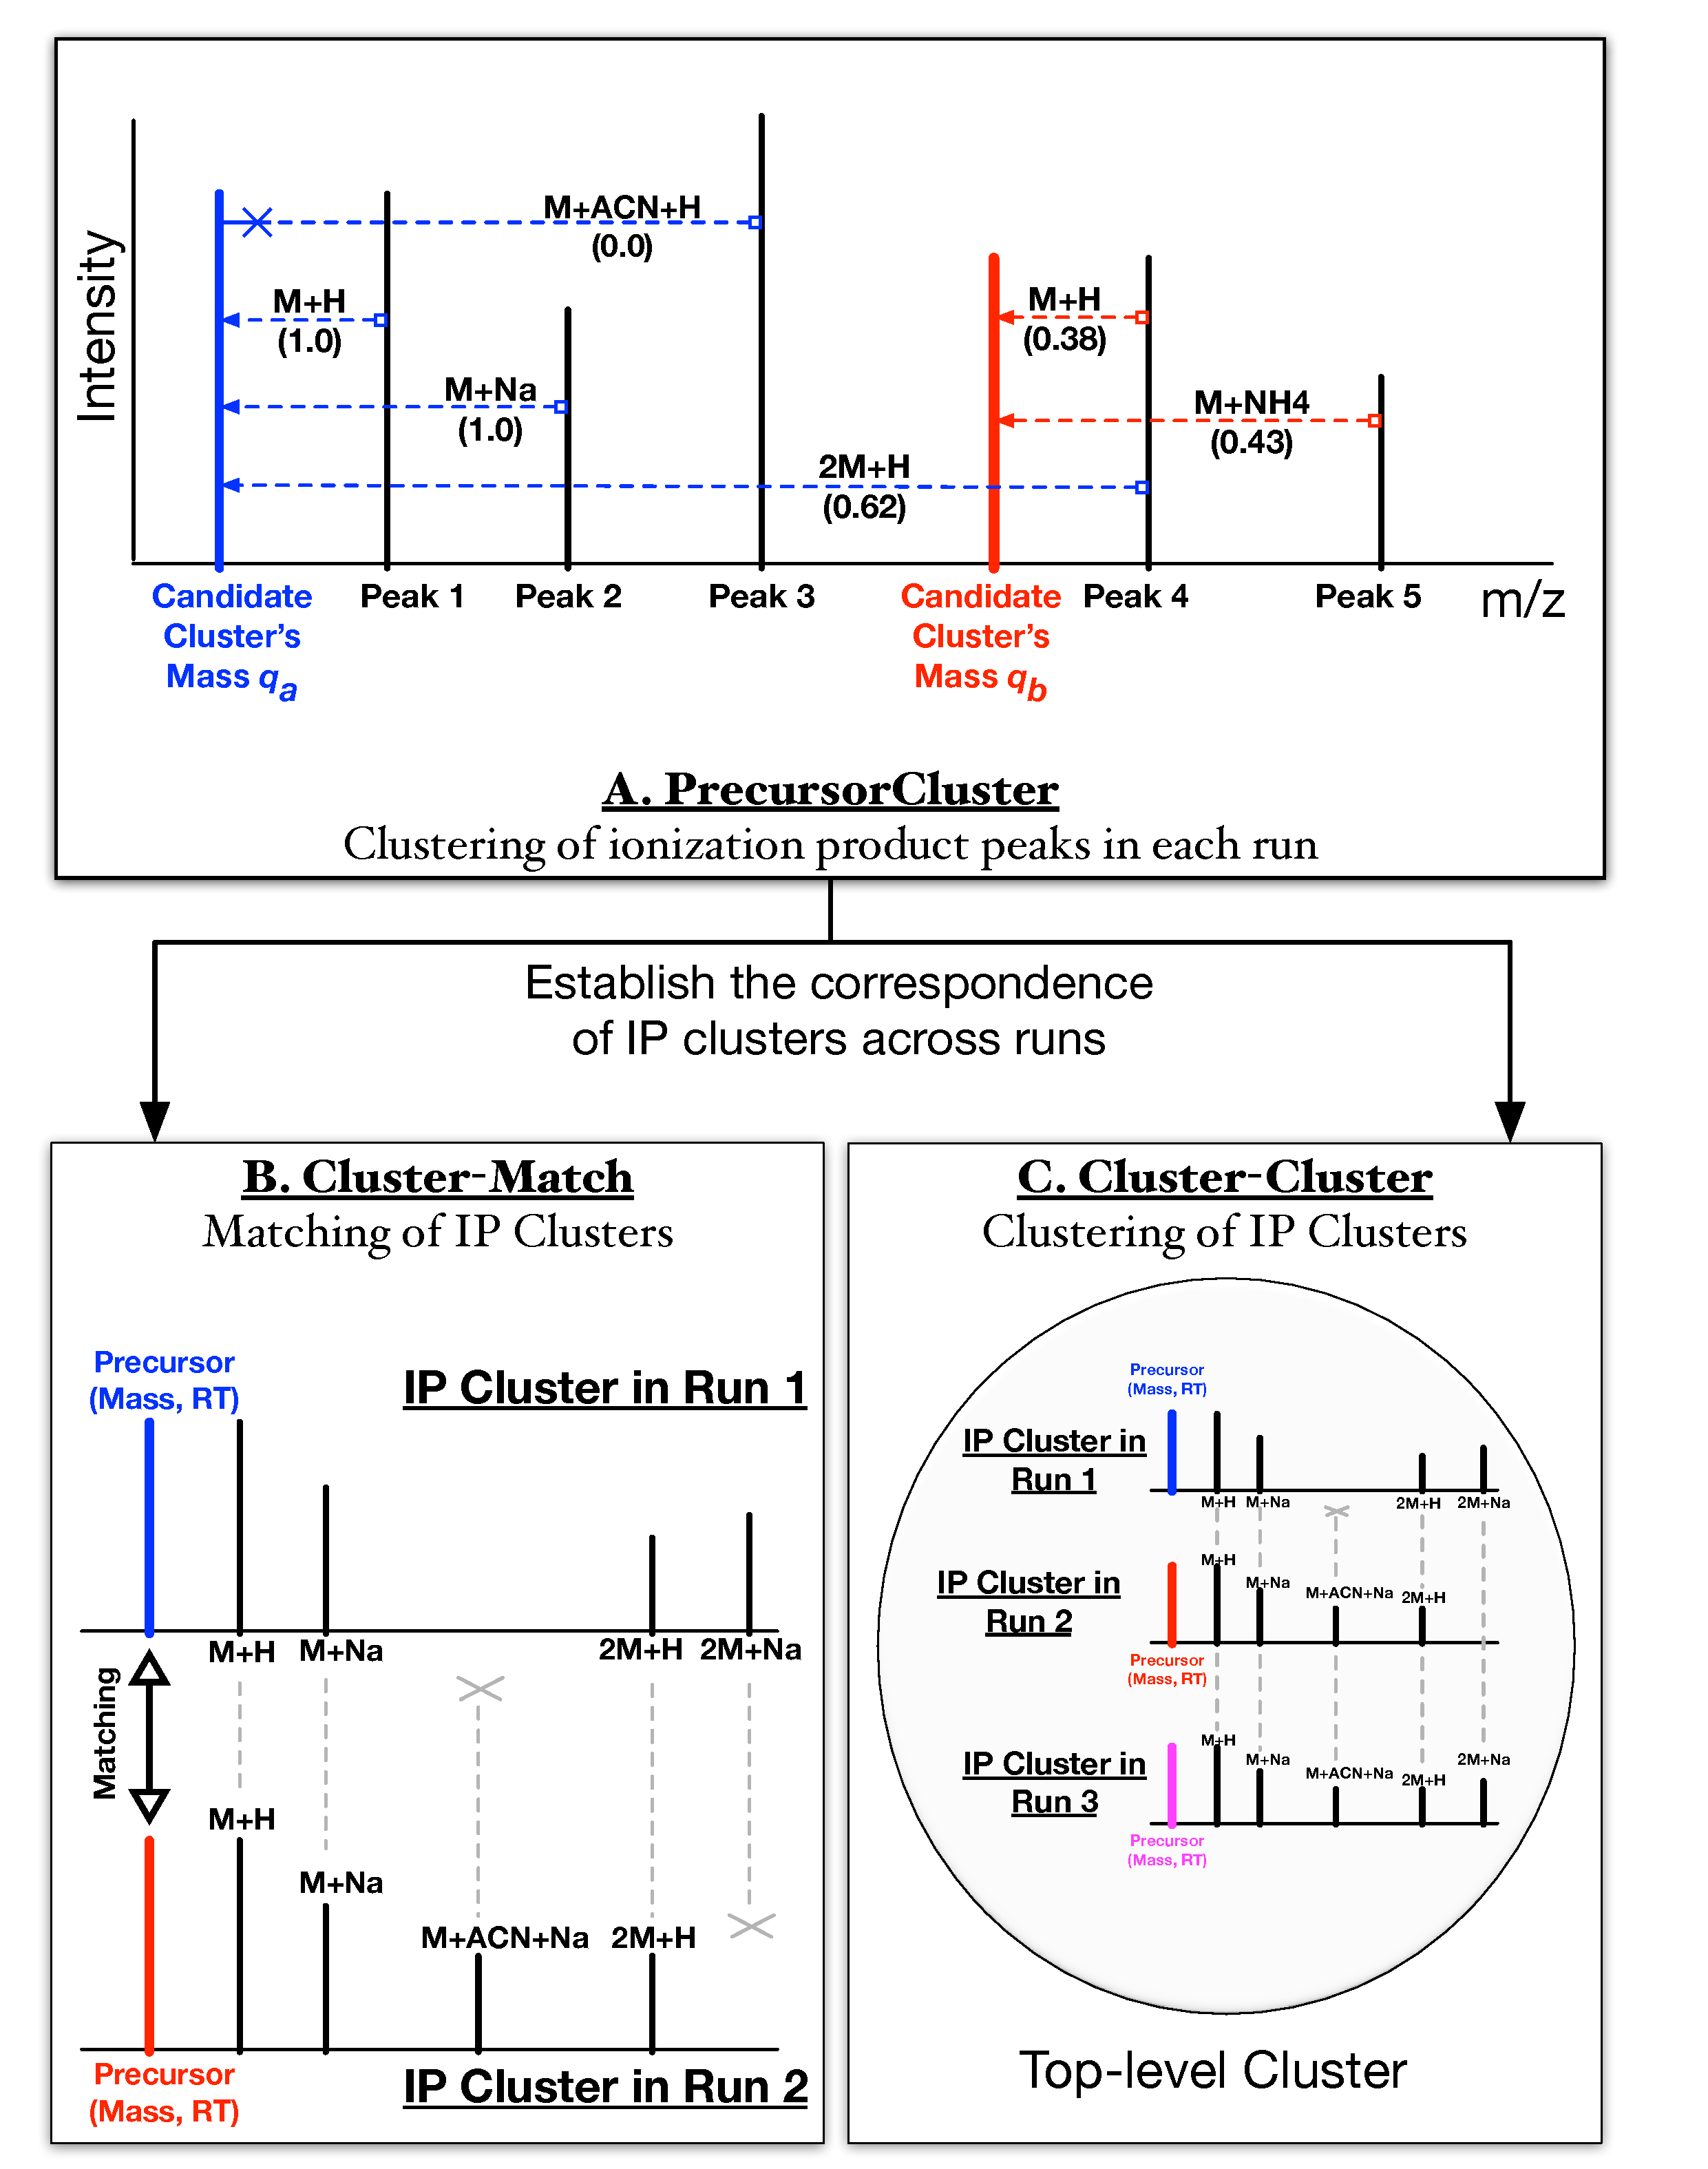
\includegraphics[width=0.75\linewidth]{05-precursor-cluster/figures/fig1.pdf}
\caption{\label{fig:01} The proposed workflow. The input to PrecursorCluster is a list of m/z, RT and intensity values. During the enumeration stage, candidate IP clusters are generated from each peak through the M+H transformation. In this example, Peak 1 and Peak 4 generate candidate IP clusters with precursor masses $q_a$ (blue) and $q_b$ (red). In the inference stage, Peak 1 and Peak 2 are clustered to $q_a$ through transformation M+H and M+Na with probabilities 1.0. Peak 3 has a valid transformation to $q_a$, but is not allowed to join that cluster since its intensity is $>$ than the intensity of the $[M+H]^+$ peak that generated the cluster (peak 1). Peak 4 can join the $q_a$ cluster through the 2M+H transformation (with probability 0.62) or form its own candidate M+H cluster having the precursor mass $q_b$ (with probability 0.38.) The latter allows for Peak 5 to join that cluster through the M+NH4 transformation (with probability 0.43). The final clustering is established by taking the \textit{maximum a posteriori} assignment for each peak feature. Non-empty IP clusters can be aligned by matching their posterior precursor mass and RT values (Fig.~\ref{fig:01}B) or through a second-stage clustering process (Fig.~\ref{fig:01}C). The correspondence of peak features in matched IP clusters is constructed by grouping peak features having the same transformation types, shown as the gray dotted lines in Figures~\ref{fig:01}B \& C.}
\end{figure}

\subsection{PrecursorCluster: clustering of ionization product peaks\label{sub:ip-clustering}}

PrecursorCluster uses a mixture model to group the multiple ionization products that arise from each metabolite. We describe and evaluate the model for the positive ionization mode data, but the method could easily be adapted to negative mode data. In a run, the $n$-th peak feature is represented as the vector $\textbf{d}_n=(d_n^m,d_n^t,d_n^p)$ with $d_n^m$ the m/z value, $d_n^t$ the RT value and $d_n^p$ the intensity value of that peak. A list of $T$ transformation functions of commonly-known IP types is also required (for e.g. see Table~\ref{Tab:transformation}). A transformation function $t_k$ takes as input the observed m/z value of a peak and produces as output the precursor mass into an IP cluster $k$ under that transformation. This takes the form of $t_k(d_n^m) = \frac{d_n^m|c|+ce-\sum_{i} h_i G_i}{n}$, where $c$ is the charge, $e$ is the mass of an electron, $n$ the multiplicity of the original molecule, and $h_i$ and $G_i$ are the count and atomic masses of the $i$th adduct part. For example, for $[M+H+NH4]^+$, $c$ is 2, $n$ is 1 while $\sum_{i} h_i G_i$ is the total atomic mass of $H+NH3$.

Although it is not strictly necessary, we found it useful \textbf{how?} to add some constraints to our mixture model. In particular, we make the assumption that an IP cluster must contain the $[M+H]^+$ ion peak and this must be the most intense peak. Although this will not always be the case, we found good performance under this assumption. These assumptions allow us to define the complete set of clusters --- one for each peak, with the precursor mass of that cluster computed via assuming the peak is an $[M+H]^+$ ion. The $k$-th cluster is represented by the tuple ($c_k^m,c_k^t,c_k^p$), where the cluster's precursor mass $c_k^m$ is the M+H transformed precursor mass of the respective peak's m/z value, and the cluster's RT ($c_k^t$) and intensity ($c_k^p$) values are the peak's RT and intensity values. Having created the set of clusters, an enumeration step is performed to determine which possible clusters each peak can belong to. A peak $\textbf{d}_n$ can be assigned to a possible cluster $k$ if \textbf{(1)} the m/z value of that peak can be transformed (through any of the $T$ transformations) into a precursor mass value that is within $\gamma_m$, the tolerance in parts-per-million (ppm), from $c_k^m$, \textbf{(2)} the RT value of that peak is within a certain tolerance ($\gamma_t$ seconds) from $c_k^t$ and \textbf{(3)} the intensity of that peak is less than the cluster's intensity threshold $c_k^p$. All observed peaks belong to at least one possible cluster (the one for which it is the $[M+H]^+$ peak).

Let $\boldsymbol{z}_{nk}$ denote the assignment of peak feature $\textbf{d}_n$ to a possible cluster $k$, i.e. $\boldsymbol{z}_{nk}$ is 1 if peak $n$ is assigned to cluster $k$ and 0 otherwise. A peak can only be assigned to exactly one cluster ($\sum_{k=1}^{K} \boldsymbol{z}_{nk}=1$). Following the standard mixture model construction, $\boldsymbol{z}_{n}$ is modelled as a multinomial distribution having the parameter vector $\boldsymbol{\theta}$, itself drawn from a prior Dirichlet distribution having the symmetric parameter $\alpha$. The likelihood of a peak $\textbf{d}_n$ being assigned to a cluster $k$ depends on the likelihood of that peak's transformed precursor mass and RT values under the possible cluster's mass and RT values. Assuming independence between mass and RT terms, this is:
% \begin{align} 
% \boldsymbol{d}_n\vert\boldsymbol{z}_{nk}=1,... &\sim L(\boldsymbol{d}_n\vert\boldsymbol{z}_{nk}=1,...) \label{eq:likelihood-short}
% \end{align}
% where $L(\boldsymbol{d}_n\vert\boldsymbol{z}_{nk}=1,...)$ is the likelihood of peak $n$ under cluster $k$ and $...$ denotes any other parameters being conditioned upon but not explicitly listed. We assume independence between mass and RT terms:
\begin{equation}\label{eq:likelihood}
p(\boldsymbol{d}_n\vert\boldsymbol{z}_{nk}=1,...)=p(t_k(d_n^m)\vert\boldsymbol{z}_{nk}=1,...) \cdot p(d_n^t\vert\boldsymbol{z}_{nk}=1,...).
\end{equation}
The likelihood of the transformed precursor mass $t_k(d_n^m)$ in the mass term $p(t(d_n^m)\vert\boldsymbol{z}_{nk}=1,...)$ in eq. (\ref{eq:likelihood}) is a product of two further terms. The first is the indicator function $I(n,t, k)$, set to 1 if no other peaks apart from $\textbf{d}_n$ are currently assigned to cluster $k$ through transformation $t$, and 0 otherwise. This allows each transformation type to appear only once in each cluster. We assume that the mass of cluster $k$, $\mu_k^m$, has a Gaussian prior with mean $c_k^m$ and fixed precision $\delta$. The precision is set to reflect the mass tolerance in parts-per-million used during the enumeration of peaks to possible clusters, such that one standard deviation ($\sqrt{\delta^{-1}}$) is $\frac{\gamma_m*c_k^m/1e6}{3}$. Within a cluster, we assume Gaussian noise in the mass, with the prior mass mean $\mu_0$ set to the value of the cluster's precursor mass $c_k^m$ used during enumeration and precision again equal to $\delta$. The mass component of the likelihood is given by:
\begin{align}
p(t_k(d_n^m)\vert\boldsymbol{z}_{nk}=1,...) &= I(n,t, k) \cdot \mathcal{N}(t_k(d_n^m) \vert \mu_k^m,\delta^{-1}) \label{eq:mass-term-pc} \\
p(\mu_k^m\vert \mu_0,\delta) &= \mathcal{N}(\mu_k^m \vert \mu_0,\delta^{-1}) \label{eq:mass-prior-pc}
\end{align}
Similarly, Gaussian noise is assumed for the RT values. The $k$-th cluster has mean RT value given by $\mu_k^t$ and precision $\lambda$ set to reflect the RT tolerance used during enumeration of possible assignments, i.e. $\gamma_t$ is $3\sqrt{\lambda^{-1}}$. Within a cluster, the noise is assumed Gaussian, with the prior RT mean $\psi_0$ set to the cluster's RT value $c_k^t$ and precision $\lambda$:
\begin{align}
p(d_n^m\vert\boldsymbol{z}_{nk}=1,\mu_k^t,\lambda) &= \mathcal{N}(d_n^m \vert \mu_k^t,\lambda^{-1}) \label{eq:rt-term-pc}\\
p(\mu_k^t\vert \psi_0,\lambda) &= \mathcal{N}(\mu_k^t \vert \psi_0,\lambda^{-1}) \label{eq:rt-prior-pc}
\end{align}
A collapsed Gibbs sampling scheme is used to infer $\boldsymbol{z}_{nk}$, the assignments of peak $n$ to cluster $k$ (details in the next section). Averaging over the posterior samples, peaks are assigned to the most likely IP cluster based on their \textit{maximum a-posteriori} (MAP) probabilities. The result from inference is the set of IP clusters, some of which may be empty and can be ignored, while others consist of related ionization products. 

PrecursorCluster can be seen as a data-reduction procedure, taking as input the set of observed peak features per run and producing as output their MAP assignments into IP clusters. Non-empty IP clusters can now take the place of individual peak features as objects to be aligned. Each IP cluster in run $j$ can be represented by $\boldsymbol{c}_{jk}=({\bar{q}}_{jk}, {\bar{r}}_{jk}, \boldsymbol{\bar{u}}_{jk})$., with ${\bar{q}}_{jk}$ the IP cluster's posterior precursor mass value, ${\bar{r}}_{jk}$ the posterior RT value and $\boldsymbol{\bar{u}}_{jk}$ the adduct `fingerprint' vector of length $T$ for that IP cluster, created after the MAP assignments of observed peaks into the cluster. This stores the binary flags on which adduct transformations bring member peaks into that IP cluster (1 if that transformation brings a peak into the cluster and 0 otherwise). These posterior mass, RT and adduct fingerprint values are used during the latter alignment stage.

\subsubsection{Gibbs Sampling for PrecursorCluster\label{sub:ip-clustering-gibbs}}

For Gibbs sampling, the conditional distribution of a peak $\boldsymbol{d}_{n}$ currently being sampled to be placed in any of the $K$ IP clusters is given by
\begin{equation}
P(z_{nk}=1|\boldsymbol{d}_{n},\ldots)\propto(\alpha_{k}+n_{k})\cdot p(\mathbf{d}_{n}|z_{nk}=1,...)\label{eq:finite_conditional}
\end{equation}
where $n_{k}$ is the current number of members (peak features) in an IP cluster $k$, $\alpha_{k}=\frac{\alpha}{K}$ the symmetric prior on the Dirichlet distribution and $p(\mathbf{d}_{n}|z_{nk}=1,...)$ is the likelihood of peak $\mathbf{d}_{n}$ in a cluster $k$. Assuming independence between the mass and RT terms, the likelihood $p(\mathbf{d}_{n}|z_{nk}=1,...)$ can be factorised into its mass and RT terms (see eq.~\ref{eq:likelihood}). However, the probability of a peak $n$ to be placed in cluster $k$ is 0 if the indicator function $I(n,t, k)$ in eq. (\ref{eq:mass-term-pc}) returns 0, i.e. another peak apart from $n$ is already assigned to cluster $k$ through transformation $t$. Otherwise, marginalising over all mixture components in eq. (\ref{eq:mass-term-pc}), the following posterior predictive distribution is obtained for the mass term: 
\begin{eqnarray}
p(t_{k}(d_{n}^{m})|z_{nk}=1...) & = & \mathcal{N}(t_{k}(d_{n}^{m})|\mu_{k},\sigma_{k}^{-1})\label{eq:mass-term}
\end{eqnarray}
where $\sigma_{k}=(\delta(1+c_{k})^{-1}+\delta^{-1})^{-1}$ and $\mu_{k}=\frac{1}{\sigma_{k}}\left[\delta(\mu_{0}+\sum_{n}t(d_{n\in k}^{m}))\right]$.
Here, $\sum_{n}t_{k}(d_{n\in k}^{m})$ denotes the sum of the transformed mass values of all the peaks (excluding the current peak being sampled) that have been assigned to cluster $k$, and $c_{k}$ the count of such peaks. Similarly, the RT term in eq.~\ref{eq:rt-term-pc} can be marginalized into
\begin{eqnarray}
p(d_{n}^{t}|z_{nk}=1...) & = & \mathcal{N}(d_{n}^{t}|\mu_{k},\sigma_{k}^{-1})\label{eq:rt-term}
\end{eqnarray}
where $\sigma_{k}=(\lambda(1+c_{k})^{-1}+\lambda^{-1})^{-1}$ and $\mu_{k}=\frac{1}{\sigma_{k}}\left[\delta(\psi_{0}+\sum_{n}d_{n\in k}^{t})\right]$, with $\sum_{n}d_{n\in k}^{t}$ denoting the sum of the RT values of all the peaks (excluding the current one) in cluster $k$.

\subsection{Cluster-Match: direct matching of ionization product clusters\label{sub:cluster-match}}

The ionization product clustering model described in Section~\ref{sub:ip-clustering} is essentially a data-reduction procedure, where within a single file $j$, the model takes as input the set of observed peaks in a single run and produces as output their groupings into IP clusters. Given the set of non-empty IP clusters and the peak features they contain, we can now treat IP clusters as a reduced set of features within a run and align (match) them across runs. We call this approach Cluster-Match. This contrasts to the conventional approach of matching all peak features directly to produce the alignment of peak features across runs. 

As detailed in Chapter~\ref{c:matching}, in the direct matching alignment of two runs, the problem of establishing the matching between two runs can be viewed as finding the maximum weighted matching in a bipartite graph, where a node in the graph represents a peak feature, an edge represents a potential matching across two sides of the graph and the edge weight is the similarity between two potential matches. The MW method  in Chapter~\ref{c:matching} is an instance of a greedy algorithm that produces an approximation of at least 1/2 of the maximum weight in the matching of a bipartite graph \cite{Maximum2011}. Only peaks that are within mass and RT tolerances from each other across runs can possibly be matched (they have an edge linking them in the graph). While simple, the results in Chapter~\ref{c:matching} shows that the MW method is generally competitive in performance to more sophisticated direct-matching methods, such as SIMA that relies on constructing stable-matching. We apply this direct matching methods to match IP clusters across runs, with IP clusters taking the place of individual peak features as nodes in the bipartite graph to be matched. The matching is therefore performed based on the precursor mass and RT values of IP clusters, rather than the observed peak's m/z and RT values. Once matching has been constructed, the alignment between the actual peak features in matched IP clusters can be established by grouping peaks that have the same transformation type across matched IP clusters (Figure~\ref{fig:01}B.)

To extend the above procedure to the alignment of multiple runs, two initial runs are first aligned to construct an intermediate merged results. Consensus features are created by taking the average m/z and RT values of matched features, and the next run is then aligned to the merged results. This procedure is repeated until all runs have been exhausted. This match-merge scheme is commonly employed by other direct matching methods \cite{Voss2011a, Pluskal2010} and requires selecting a reference run. In practice, the choice of reference run is arbitrary and its effect has not been fully investigated (in our implementation, the first run in alphabetical sorting is used as the reference run and the same ordering of runs is always used for all methods compared.)

\subsection{Cluster-Cluster: across-run clustering of ionization product clusters\label{sub:cluster-cluster}}

The proposed pairwise matching scheme used by Cluster-Match is frequently extended to the processing of multiple runs in a fairly ad-hoc manner (as seen in the match-merge approach at the end of Section~\ref{sub:cluster-match}, also commonly used by other direct matching tools). This approach suffers from the limitation of having to set a reference run for the matching and consequently, the fact that altering the ordering of runs to be processed might change the alignment results \cite{Smith2013}. The alternative approach of generalizing from pairwise matching in a bipartite graph into finding the maximum weighted matching in a general graph is typically a computationally expensive operation. Producing a distance measure that works well for measuring similarities of peaks across runs is a non-trivial problem, and such matching procedures, whether through successive pairwise merging or operating on a general graph, generally do not take into account the uncertainties in the matching of peak features across runs.

Here, we propose using another clustering procedure (Cluster-Cluster) to further cluster the IP clusters produced from the first-stage IP clustering in Section~\ref{sub:ip-clustering}. In this manner, IP clusters coming from different runs are further clustered into top-level clusters shared across runs (Figure~\ref{fig:01}C). The actual alignment of peak features can then be established by \textbf{(1)} looking at which IP clusters are put together into the same top-level cluster (essentially, their matching) and \textbf{(2)} in a top-level cluster, grouping peak features from different runs that have the same transformation type to establish their alignments. In this scheme, there is no need to set a reference run. Crucially, the posterior probabilities of certain IP clusters being assigned into the same top-level cluster provides us with an estimate of matching confidence of peak features.

Only peaks within a certain across-run mass tolerance should be matched, so a partitioning of IP clusters into top-level bins is performed. Across all runs $j=1,...,J$, IP clusters are sorted by their posterior mass values $\{{\bar{q}}_{jk}\}$. The smallest unprocessed mass value $min(\{{\bar{q}}_{jk}\})$ is used to initialize a top-level bin. Subsequent IP clusters (in ascending mass order) are grouped into the bin until an IP cluster with a posterior mass that differs by $\gamma'_m$ ppm (a user-defined mass tolerance across runs) from $min(\{{\bar{q}}_{jk}\})$ is encountered, in which case, a new top-level bin is started using that cluster. The process is repeated until all IP clusters are processed.

If a top-level bin contains only one IP cluster, no possible matching can be constructed, otherwise IP clusters in the same bin can potentially be clustered (into top-level clusters) and therefore matched. To avoid specifying the number of top-level clusters \textit{a priori}, we use an infinite Gaussian mixture model, described in Chapter~\ref{c:ml-background}, to model the data. Let $\boldsymbol{\bar{z}}_{jki}=1$ denote the assignment of IP cluster $k$ coming from file $j$ into top-level cluster $i$.

Then:
\begin{align}
\boldsymbol{\pi}\vert\alpha' &\sim GEM(\alpha') \\
\boldsymbol{\bar{z}}_{jk}\vert\boldsymbol{\pi} &\sim Multinomial(\boldsymbol{\pi}) \\
\boldsymbol{c}_{jk}\vert\boldsymbol{\bar{z}}_{jki}=1,... &\sim p(\boldsymbol{c}_{jk}\vert\boldsymbol{\bar{z}}_{jki}=1,...)
\end{align}
where $\boldsymbol{\pi}$ are the mixing proportions, distributed according to the GEM (Griffiths, Engen and McCloskey) distribution (details in Chapter~\ref{c:ml-background}). The likelihood of $\boldsymbol{c}_{jk}$, the $k$-th IP cluster from run $j$, to be placed in a top-level cluster $i$ is assumed to be factorized into independent factors of its mass, RT and adduct signature terms:
\begin{equation}\label{eq:second-stage-likelihood}
\begin{split}
p(\boldsymbol{c}_{jk}\vert\boldsymbol{\bar{z}}_{jki}=1,...) = p({\bar{q}}_{jk}\vert\boldsymbol{\bar{z}}_{jki}=1,...) \cdot p({\bar{r}}_{jk}\vert\boldsymbol{\bar{z}}_{jki}=1,...) \cdot \\
p({\boldsymbol{\bar{u}}}_{jk}\vert\boldsymbol{\bar{z}}_{jki}=1,...)
\end{split}
\end{equation}
In eq. (\ref{eq:second-stage-likelihood}), the mass term $p({\bar{q}}_{jk}\vert\boldsymbol{\bar{z}}_{jki}=1,...)$ is defined analogously to the first-stage clustering step (Section~\ref{sub:ip-clustering}). The indicator function $\bar{I}(k,j,i)$ in eq. (\ref{eq:second-mass-term}) is set to 1 if there are no other IP clusters from run $j$, apart from the $k$-th IP cluster, that are assigned to the $i$-th top-level cluster, and 0 otherwise. This ensures that there is at most one IP cluster from each run assigned to a top-level cluster. The IP cluster posterior mass ${\bar{q}}_{jk}$ is distributed according to a Gaussian distribution with mean $c_m$ and precision $\bar{\delta}$, where the across-run mass tolerance $\gamma'_m$ is set to be equivalent to 3 standard deviations in ppm. The mass of top level cluster $c_m$ is in turn drawn from a base Gaussian distribution having prior mass mean $\bar{\mu}_0$ and precision $\sigma_m$ (eq. \ref{eq:second-mass-prior}). The $\bar{\mu}_0$ parameter is set to the mean of the posterior m/z values of the IP clusters in the top-level bin, while $\sigma_m$ is set to a broad value of 5E-3. 
\begin{align}
p({\bar{q}}_{jk}\vert\boldsymbol{\bar{z}}_{jki}=1,c_m,\bar{\delta},...) &= \bar{I}(j,i) \cdot \mathcal{N}(\bar{q}_{jk} \vert c_m,\bar{\delta}^{-1}) \label{eq:second-mass-term}\\
p(c_m\vert \bar{\mu}_0,\sigma_m) &= \mathcal{N}(c_m \vert \bar{\mu}_0,\sigma_m^{-1}) \label{eq:second-mass-prior}
\end{align}
In the RT term $p({\bar{r}}_{jk}\vert\boldsymbol{\bar{z}}_{jki}=1,...)$, ${\bar{r}}_{jk}$ is distributed according to a Gaussian distribution with mean $c_t$ and precision $\bar{\lambda}$ (eq. \ref{eq:second-rt-term}). Again, the across-run RT tolerance $\gamma'_t$ is set to be equivalent to 3 standard deviations in seconds. The same uninformative parameter values are set on the prior RT mean parameter $\bar{\psi}_0$ and precision $\sigma_t$ (eq. \ref{eq:second-rt-prior}).
\begin{align}
p({\bar{r}}_{jk}\vert\boldsymbol{z}_{jki}=1,c_t,\bar{\lambda}) &= \mathcal{N}({\bar{r}}_{jk} \vert c_t,\bar{\lambda}^{-1}) \label{eq:second-rt-term}\\
p(c_t\vert \bar{\psi}_0,\sigma_t) &= \mathcal{N}(c_t \vert \bar{\psi}_0,\sigma_t^{-1}) \label{eq:second-rt-prior}
\end{align}
Finally, in the adduct fingerprint term $p({\boldsymbol{\bar{u}}}_{jk}\vert\boldsymbol{z}_{jki}=1,...)$, the vector ${\boldsymbol{\bar{u}}}_{jk}$ is modelled using a multinomial distribution having a Dirichlet prior with symmetric hyper-parameter $\beta$.
% \begin{align}
% \boldsymbol{\psi}\vert\beta &\sim Dir(\beta) \label{eq:second-fingerprint-prior}\\
% {\boldsymbol{\bar{u}}}_{jk}\vert\boldsymbol{\psi} &\sim Multinomial(\boldsymbol{\psi}) \label{eq:second-fingerprint-like}
% \end{align}
The entire likelihood function of eq. \ref{eq:second-stage-likelihood} ensures that IP clusters from different runs are placed in a single top-level cluster if: \textbf{(1)} they are from different runs, \textbf{(2)} they share similar posterior precursor mass and RT values, and \textbf{(3)} they have similar adduct fingerprint. Inference on model parameters is again performed via Gibbs sampling. Within each posterior sample, peak features in matched IP clusters sharing the same transformation type are grouped (Figure~\ref{fig:01}C), forming aligned peaksets. The occurrences of aligned peaksets are counted and averaged across samples to give matching confidences.

\subsubsection{Gibbs Sampling for Cluster-Cluster\label{sub:cluster-cluster-gibbs}}

Analytical inference is not tractable here, so we use a collapsed Gibbs sampling scheme for inference of Cluster-Cluster. The conditional probability of $P(\boldsymbol{\bar{z}}_{jki}=1\vert...)$ of IP cluster $k$ in file $j$ to be placed in an existing top-level cluster $i$ (or $i^{*}$ if a new top-level cluster is to be created), is given by:
\begin{equation}
P(\boldsymbol{\bar{z}}_{jki}=1|\boldsymbol{c}_{jk},\ldots)\propto\begin{cases}
\begin{array}{c}
n_{i}\cdot p(\boldsymbol{c}_{jk}|\boldsymbol{\bar{z}}_{jki}=1,...)\\
\alpha'\cdot p(\boldsymbol{c}_{jk}|\boldsymbol{\bar{z}}_{jki^{*}}=1,...)
\end{array}\end{cases}\label{eq:table_likelihood-cc}
\end{equation}
where $n_{i}$ is the current number of members (IP clusters) in an existing top-level cluster $i$. $p(\mathbf{y}_{n}|z_{nk}=1,...)$ is the likelihood of peak $\mathbf{y}_{n}$ in an existing cluster $k$. The top part of eq. (\ref{eq:table_likelihood-cc}) is the conditional probability on existing mixture components of the model, and can be factorized into its independent mass, RT and adduct fingerprint terms. The bottom part of eq. (\ref{eq:table_likelihood-cc}) represent new components that are created as needed. 
\begin{enumerate}
\item For the mass term $p({\bar{q}}_{jk}\vert\boldsymbol{\bar{z}}_{jki}=1,...)$, we obtain the following predictive distribution after marginalizing over all mixture components: \begin{eqnarray} p({\bar{q}}_{jk}\vert\boldsymbol{\bar{z}}_{jki}=1,...) & = & \mathcal{N}({\bar{q}}_{jk}|\mu_{k},\gamma_{k}^{-1})\label{eq:15-2} \end{eqnarray} where $\gamma_{k}=((\sigma_{m}+\bar{\delta}n_{i})^{-1}+\bar{\delta}^{-1})^{-1}$ and $\mu_{k}=\frac{1}{\gamma_{k}}\left[(\sigma_{m}\bar{\mu}_{0})+(\bar{\delta}\sum_{j}\sum_{k}\bar{q}_{jk\in i})\right]$. Note that in the summation terms of $\mu_{k}$, $\sum_{j}\sum_{k}\bar{q}_{jk\in i}$ denotes the sum of posterior mass values of IP clusters currently assigned to top-level cluster $i$ (excluding the current IP cluster being sampled), and $n_{i}$ the count of such IP clusters. 
\item Similarly, the RT term $p({\bar{r}}_{jk}\vert\boldsymbol{\bar{z}}_{jki}=1,...)$ can be marginalized into a Gaussian with precision $\gamma_{k}=((\sigma_{t}+\bar{\lambda}n_{i})^{-1}+\bar{\lambda}^{-1})^{-1}$ and mean $\mu_{k}=\frac{1}{\gamma_{k}}\left[(\sigma_{t}\bar{\psi}_{0})+(\bar{\lambda}\sum_{j}\sum_{k}\bar{r}_{jk\in i})\right]$, with $\sum_{j}\sum_{k}\bar{r}_{jk\in i}$ the sum of posterior RT values of member IP clusters in top-level cluster $i$, excluding the current IP cluster being sampled.
\item Lastly for the adduct fingerprint term $p({\boldsymbol{\bar{u}}}_{jk}\vert\boldsymbol{\bar{z}}_{jki}=1,...)$, we marginalize over the mixture components and obtain $\frac{C\left({\boldsymbol{\bar{u}}}_{jk}+\sum_{j}\sum_{k}\boldsymbol{\bar{u}}_{jk\in i}+\boldsymbol{\beta}\right)}{C\left(\sum_{j}\sum_{k}\boldsymbol{\bar{u}}_{jk\in i}+\boldsymbol{\beta}\right)}$ with $\sum_{j}\sum_{k}\boldsymbol{\bar{u}}_{jk\in i}$ the sum of all adduct fingerprint vectors currently assigned to top-level cluster $i$ (excluding the current IP cluster being sampled), $C(\boldsymbol{X})=\frac{\prod_{j=1}^{m}\Gamma(\boldsymbol{X}_{j})}{\Gamma(\sum_{j=1}^{m}\boldsymbol{X}_{j})}$ and $\Gamma$ the gamma function.
\end{enumerate}
For new components, marginalising over the base distributions for the mass term results in a Gaussian with mean $\bar{\mu_{0}}$ and precision $\bar{\delta}^{-1}+\sigma_{m}^{-1}$. Similarly, for the RT term, this results in a Gaussian with mean $\bar{\psi_{0}}$ and precision $\bar{\lambda}^{-1}+\sigma_{t}^{-1}$. For the adduct term, this results in $\frac{C\left({\boldsymbol{\bar{u}}}_{jk}+\boldsymbol{\beta}\right)}{C\left(\boldsymbol{\beta}\right)}$.

\section{Evaluation Study}

\subsection{Evaluation Datasets}

Two metabolomics datasets were used for performance evaluation. The Standard dataset was generated from a mixture of 104 standard metabolites used for chromatographic columns calibration and has been used for performance evaluation in in Chapter~\ref{c:matching}. This dataset contains eleven runs and represents a challenging alignment scenario with large RT variability (runs were separated by weeks and generated from different instruments). A Beer dataset of three runs from one batch that is representative of the typical biochemical diversity in a complex metabolomics study is introduced. All runs were processed through PrecursorCluster using the same parameters and the list of transformations in Table~\ref{Tab:transformation}. This list includes the common adduct transformations in positive ionisation mode, but optionally isotopes can also be included.

Alignment ground truth for both datasets was constructed from the putative identification of each run at 3 ppm using the Identify module from mzMatch \cite{Scheltema2011}, taking as input a database of the 104 standard compounds known to be present and the transformations in Table~\ref{Tab:transformation}. Peak features with the same unique identifications are matched across runs, resulting in an alignment ground truth for a subset of all peaks. Only peaks present in the ground truth are considered for evaluation. The Standard ground truth accounts for 304 aligned peaksets (the set of peak features matched across runs) spanning 1936 peak features across all Standard runs, while the Beer ground truth consists of 108 aligned peaksets of 300 peak features across all Beer runs.

\begin{table}[!htbp]
\caption{List of common adduct transformations in positive mode used for the precursor clustering of the Standard and Beer runs.\label{Tab:transformation}}{\begin{tabular}{@{}lllll@{}}
M+2H & M+H & M+ACN+H & 2M+Na & M+H+NH4\\
M+NH4 & M+ACN+Na & 2M+ACN+H & M+ACN+2H & M+Na\\
M+2ACN+H & M+2ACN+2H & M+CH3OH+H & 2M+H
\end{tabular}}{}
\end{table}

\subsection{Performance Measures}

Precision and recall are widely used to evaluate alignment performance \cite{Lange2008, Pluskal2010, Ballardini2011, Voss2011a, Sandin2013}, also in Chapter~\ref{c:matching}. To evaluate alignment performance on multiple runs, we propose a generalized definition of precision and recall that extends from the pairwise definition in Chapter~\ref{c:matching}. From an alignment method or the ground truth, a list of aligned peaksets is obtained. For example, an alignment method returns a list of two aligned peaksets $\{a,b,c,d,\},\allowbreak\{e,f,g\}$ as output. When $l=2$ \textbf{first mentio of l?}, this output can be enumerated into a list of 9 `alignment items' of all the pairwise combinations of features: $\{a,b\},\allowbreak\{a,c\},\allowbreak\{a,d\},\allowbreak\{b,c\},\allowbreak\{b,d\},\allowbreak\{c,d\},\allowbreak\{e,f\},\allowbreak\{e,g\},\allowbreak\{f,g\}$. Let $M$ and $G$ be the results from such enumeration from a method's output and the ground truth respectively. Each distinct combination of features in $M$ and $G$ can be considered as an item during performance evaluation. Intuitively, the choice of $l$ reflects the strictness of what is considered to be a true positive item, with larger values of $l$ demanding an alignment method that produces results spanning more runs correctly. In this manner, $l$ goes from 2 to as many runs being aligned.

For a given $l$, the following positive and negative instances of alignment item can now be defined for the purpose of performance evaluation:
\begin{itemize}
\item True Positive ($\boldsymbol{TP}$): items that should be aligned (present in $G$) and are aligned (present in $M$).
\item False Positive ($\boldsymbol{FP}$): items that should not be aligned (absent from $G$) but are aligned (present in $M$).
\item True Negative ($\boldsymbol{TN}$): items that should not be aligned (absent from $G$) and are not aligned (absent from $M$).
\item False Negative ($\boldsymbol{FN}$): items that should be aligned (present in $G$) but are not aligned (absent from $M$).
\end{itemize}

In the context of alignment performance, precision ($\frac{\boldsymbol{TP}}{\boldsymbol{TP}+\boldsymbol{FP}}$) is therefore the fraction of alignment items in $M$ that are correct with respect to some alignment ground truth $G$, while recall ($\frac{\boldsymbol{TP}}{\boldsymbol{TP}+\boldsymbol{FN}}$) is the fraction of alignment items specified in $G$ that are actually aligned in the alignment results $M$. By definition, a perfect alignment method would have precision and recall scores of 1. In practice, there is a trade-off between precision and recall, where increasing recall often results in lower precision and vice versa. To summarize these two numbers, we also report the F$_1$ score, which is the harmonic mean of precision and recall, defined as $F_1 = 2(precision\cdot recall)/(precision + recall)$. Since our alignment ground truth is usually smaller than the set of all pairs of peaks returned by a method, only those peaks present in the ground truth are considered for evaluation. 

\subsection{Evaluation Procedure\label{sub:evaluation_procedure}}

As the baselines for evaluation, we compare the performance of our proposed methods against the method of direct matching of peak features (MW) and its variant (MWG) that modifies the similarity matrix used during matching to bring together group of peaks related by RT closer during matching -- described in Chapter~\ref{c:matching}. 

To evaluate Cluster-Match, the procedure in Chapter~\ref{c:matching} is followed. 30 random pairs of Standard runs were selected as the training set, and another 30 as the testing set. Matching tolerance parameters were varied within reasonable ranges (details in Section~\ref{sub:parameters}) on one pair in the training set, and parameters resulting in the best training performance (highest $F_1$-score) of one pair were used to align the associated pair in the testing set. The three Beer runs are too few to allow separation into training and testing sets, so each method is trained and evaluated on all three Beer runs. The direct matching of peak features (MW) and its variant (MWG) from in Chapter~\ref{c:matching} that incorporates grouping information (based on RT and not mass) into the similarity matrix used for matching are used as a baseline. 

To evaluate Cluster-Cluster, five sets of 2, 3, and 4 Standard runs were selected randomly as well as all 3 Beer runs. For each data set, parameters for Cluster-Match were varied to obtain the best attainable alignment performance. These are plotted alongside the results from Cluster-Cluster on the same data using a fixed (and potentially non-optimal) set of parameters. Cluster-Cluster was also run with and without the adduct fingerprint term to evaluate its importance. More details on parameter optimization can be found in Section~\ref{sub:parameters}.

\subsection{Parameter Optimization\label{sub:parameters}}

Following the parameter optimization procedure in Section~\ref{sub:parameters-optimisation}, the same grid search on the m/z and Rt window tolerance parameters is used.  The m/z and RT window tolerance parameters define the maximum deviation acceptable for a candidate matching is allowed in the bipartite graph. The choice of m/z parameter is often determined by the accuracy of the mass spectrometry instrument and can be reasonably determined in advance. Due to RT drift, selecting the RT window is less straightforward. 

For the evaluation of feature matching (MW, MWG) vs. cluster matching (Cluster-Match) on the Standard dataset, we performed grid-search on the m/z and RT windows parameters using the training set. The optimal training parameters are used to perform alignment on the testing set, giving the respective performance measures (testing Precision, Recall, F$_{1})$. On the Standard datasets, we varied the mass tolerance window of the methods tested within the range $\{2,4,6,8,10\}$ m/z and the RT tolerance window within $\{5,10,15,...,100\}$ seconds during the training stage. Parameter combinations that result in the best F1-score were then used for performance evaluation in the testing stage. For MWG, additional parameters are also required for the threshold $t_{g}$ on greedy clustering of related peaks and $\alpha_{g}$, the contribution on the different parts to the similarity score. We let $t_{g}$ vary within $\{2,4,6,8,10\}$ seconds and $\alpha_{g}$ within $\{0,0.2,0.4,0.6,1.0\}$ in the training stage and use the best combinations of parameter values for the testing stage. The three Beer runs are too few to allow separation into training and testing sets, so each method is trained and evaluated on all three Beer runs using the previously-described parameters same as the Standards.

The following parameters were used for the first-stage clustering of the PrecursorCluster model for all the Standard runs being processed: within-run mass tolerance $\gamma_m=5$ ppm, within-run RT tolerance $\gamma_t=30$ seconds. For the Beer runs, we used the within-run mass tolerance $\gamma_m=3$ ppm and the within-run RT tolerance $\gamma_t=10$ seconds. The prior on the Dirichlet distribution $\alpha$ is set to 1.0 and Table~\ref{Tab:transformation} shows the list of common adduct transformations in positive ionization mode used for precursor clustering. 5000 posterior samples were obtained from Gibbs sampling.

For the second-stage clustering in Cluster-Cluster, the following parameters were used for all input Standard and Beer runs: across-run mass tolerance $\gamma'_m=10$ ppm, across-run RT tolerance $\gamma'_t=60$ seconds, $\alpha'$ the Dirichlet Process concentration parameter is set to 1000.0. As relatively few number of runs are being aligned in our experiments, the large value of $alpha'$ encourages more top-level clusters, each having fewer member IP clusters inside.  $\beta$, the symmetric prior on the Dirichlet prior distribution for adduct signature vector is set to 0.1. Inference is performed on each top-level bin that has more than 1 IP clusters inside, with 500 posterior samples drawn for each top-level bin.

\section{Results and Discussions}

With PrecursorCluster, the large number of peaks present within a single LC-MS run can now be reduced to a smaller number of IP clusters, making alignment easier as fewer objects have to be matched across runs. Section~\ref{sub:precursor-cluster-results} presents the results of running the ionization product clustering on the Standard and Beer datasets. 

While the resulting IP clusters potentially have many uses (e.g. to the problem of annotation of related peaks and the identification of metabolites), peaks assigned to any IP cluster have now been annotated with the transformation type that brings them into the clusters. IP clusters can therefore be aligned across runs (through direct-matching or a second-stage clustering process) and their member peak features (sharing the same transformation type) matched to produce alignment. Section~\ref{sub:cluster-match-results} demonstrated from our experiments how the proposed approach of direct-matching IP clusters can improve upon the matching of LC-MS peak features alone, while Section~\ref{sub:cluster-cluster-results} describes how the resulting probabilities from Cluster-Cluster can be used to robustly quantify the matching uncertainties.

Being a direct matching method, Cluster-Match performs nearly as fast as alignment by matching of peak features alone while offering better performance. As Cluster-Cluster performs Bayesian inference on which IP clusters should be put together into the same top-level clusters, the alignment of LC-MS features can now be established without the need for a reference run. While this requires more computational time than the direct-matching alternative (Section~\ref{sub:running-time}), Cluster-Cluster is able to produce confidence scores on the matching quality of aligned peaksets from the posterior summaries computed during inference. This has a potential use in assisting the selection of high-confident aligned peaksets for subsequent analysis in the latter stage of the LC-MS pipeline

\subsection{Ionization Product Clustering from PrecursorCluster\label{sub:precursor-cluster-results}}

\begin{figure}[!htbp]
\centering
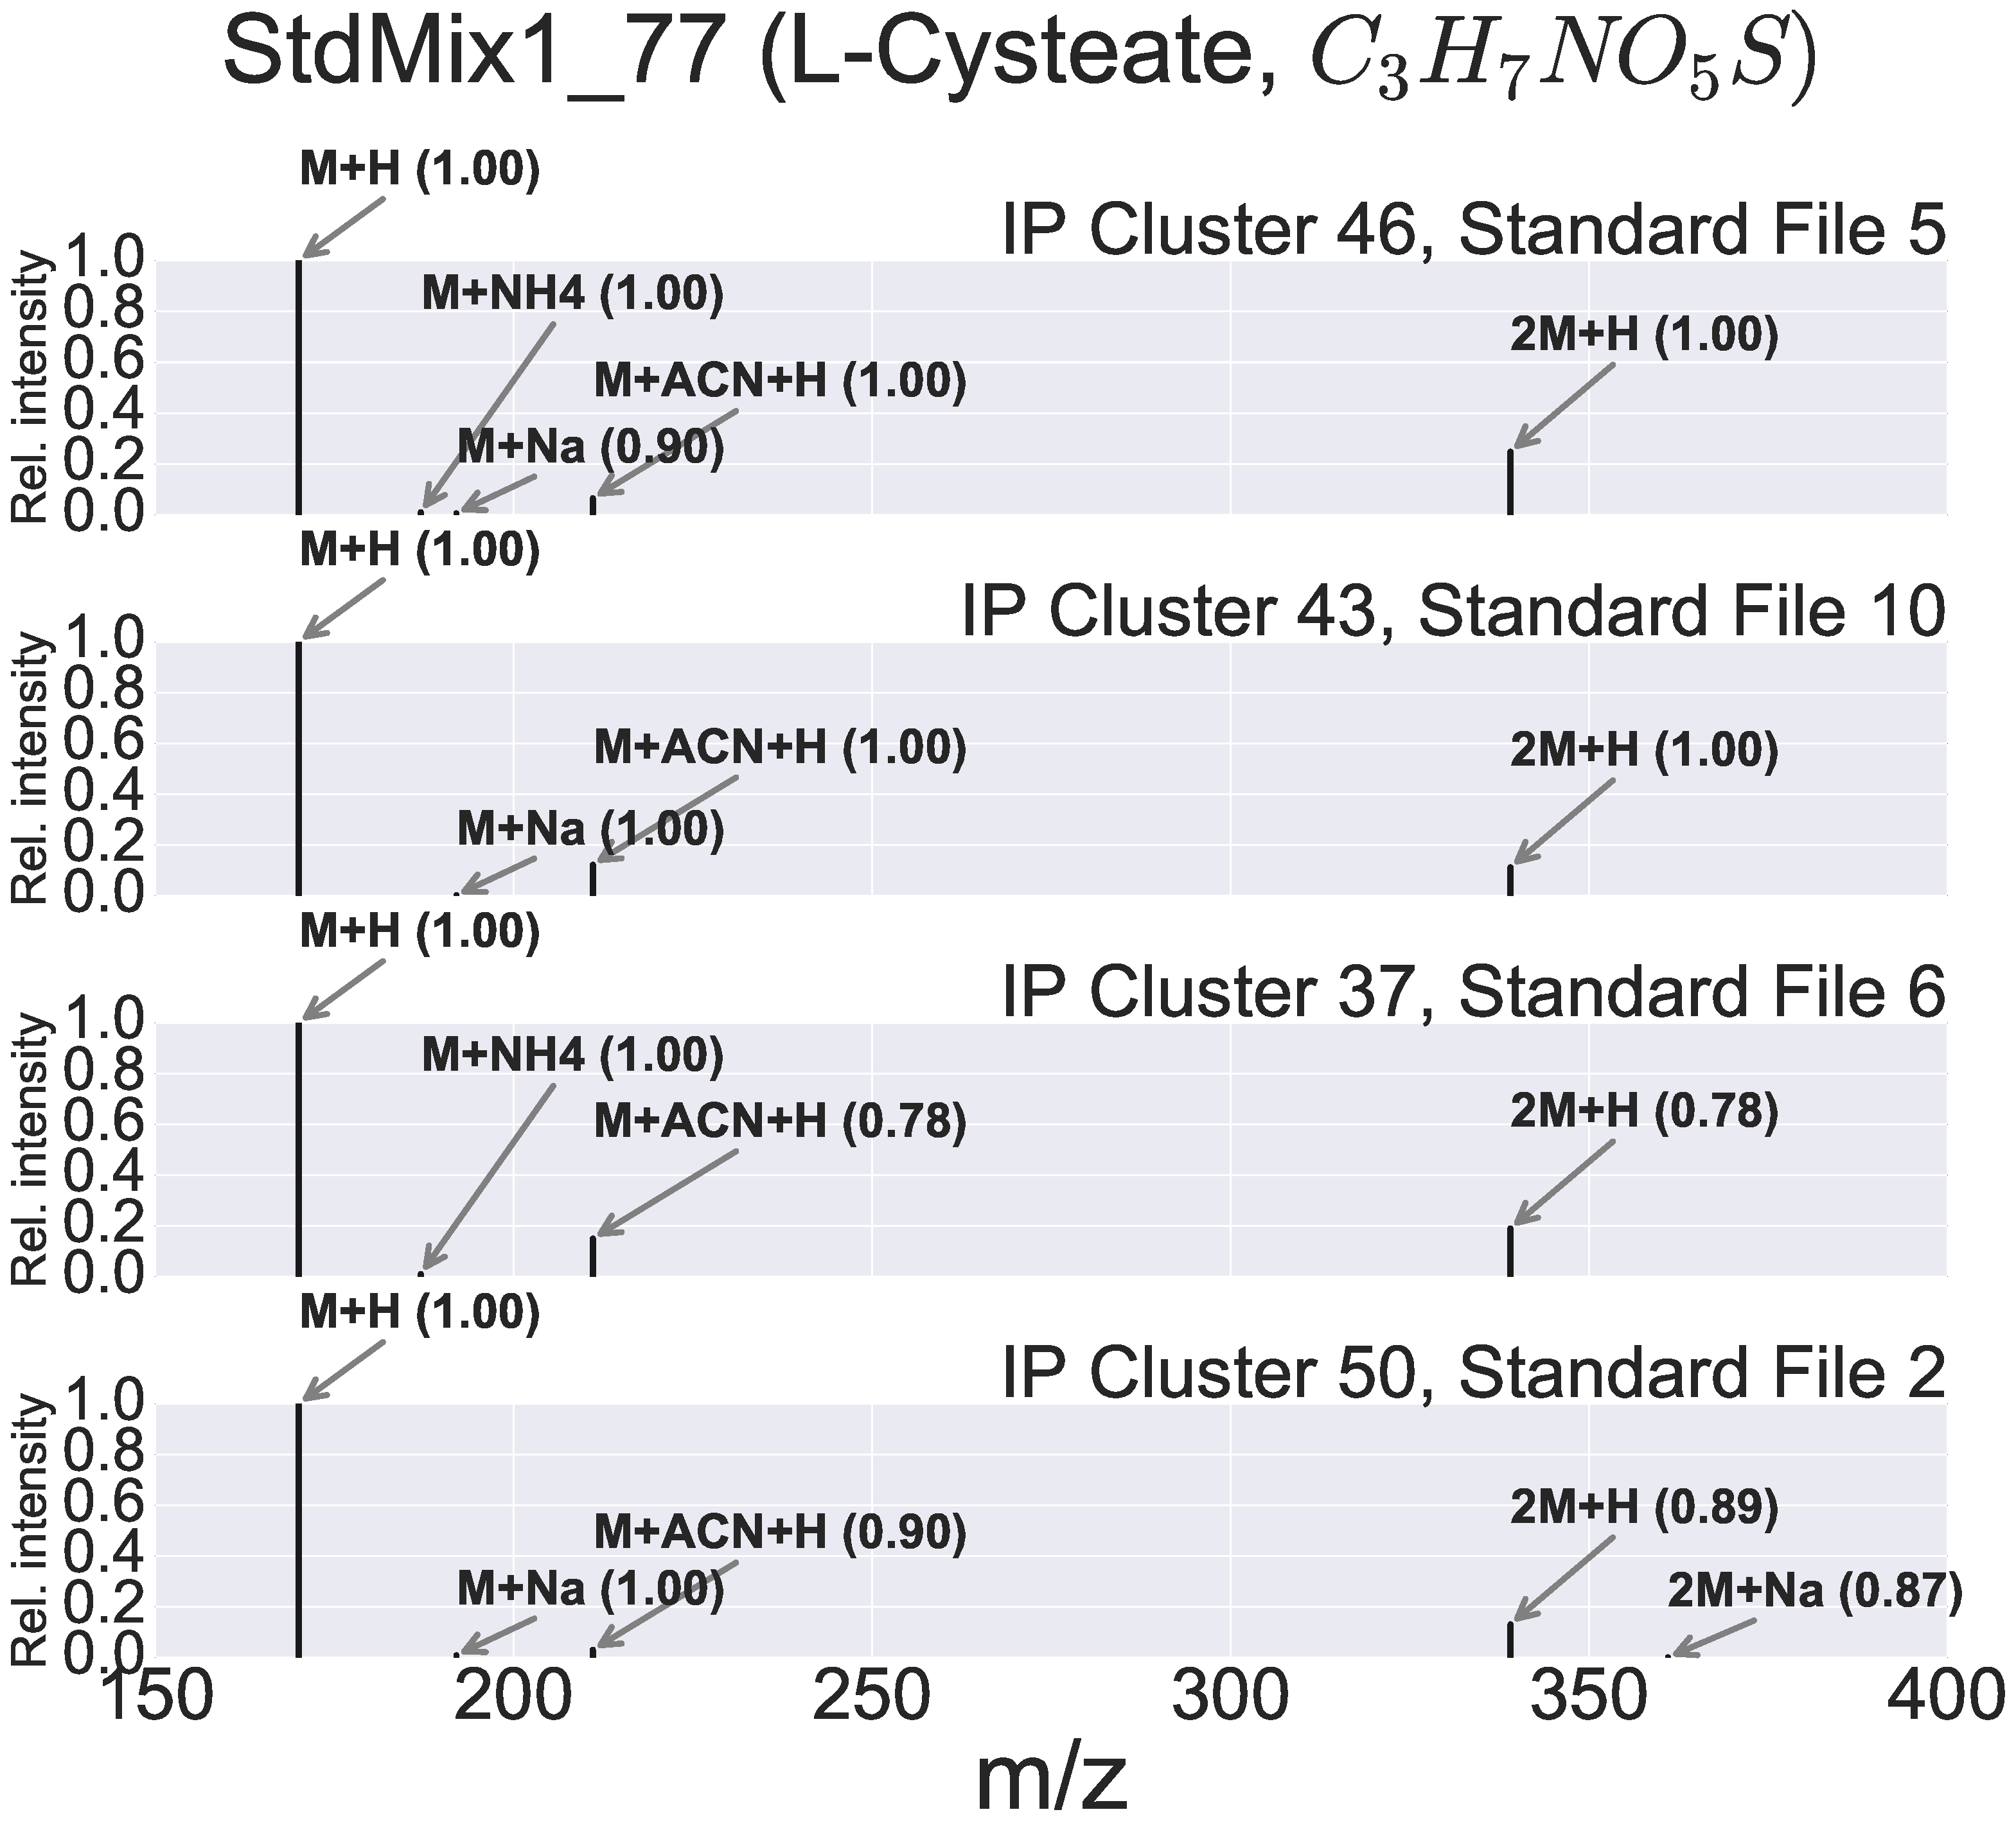
\includegraphics[width=0.6\linewidth]{05-precursor-cluster/figures/l_cysteate.eps}
\caption{\label{fig:06} Different IP clusters (46, 32, 37, 50) in four different Standard runs, identified as Cysteic acid. The MAP transformation type of a peak and its probability are annotated as a labelled arrow and the bracketed number beside. According to the ground truth, all member peaks with the same transformation type should be aligned.}
\end{figure}

Within each run, PrecursorCluster produces the \textit{maximum a posteriori} (MAP) assignments of peaks to IP clusters. An example of four IP clusters found in the Standard runs, identified as Cysteic acid, is shown in Figure~\ref{fig:06}. According to the ground truth, all member peaks across these four clusters should be aligned. Table~\ref{Tab:cluster-counts} shows that within each run, a large number of peak features cannot be clustered to other peaks within the same run and can therefore only form an IP cluster with itself as the only member through the M+H transformation (we call these clusters of only one member peak the singleton IP clusters). In both the Standard and Beer runs, non-singleton IP clusters (containing more than one member peaks) comprise approximately 6\% to 10\% of the total IP clusters of that run. The distributions of the cluster sizes of these non-singleton clusters when only adduct transformations are used are given in Figure~\ref{fig:cluster-counts} for the Standard and Beer runs. We also note that for any given cluster size, the counts of IP clusters of that size tend to differ significantly across the Standard runs, due to the varying number of LC-MS peak features present in each Standard run. This is the consequence of the Standard runs being produced in several batches separated over a period of time. The distributions of cluster sizes in Figure~\ref{fig:cluster-counts} across the three Beer runs are more consistently reproduced, reflecting the fact that the runs were generated within the same batch. As shown in Figure~\ref{fig:cluster-counts}, the largest IP clusters of the Beer and Standard runs have 6 and 7 member peaks respectively. 

\begin{table}[!htbp]
\centering
\caption{The number of peak features and the counts of singleton and non-singleton IP clusters in each run of the Standard and Beer datasets. A singleton cluster is defined to be an IP cluster having only one member peak after MAP assignments, while a non-singleton IP cluster has more than one member peaks. The last column in the Table shows the counts of non-singleton IP clusters and also the percentage of non-singleton IP clusters from the total IP clusters in that run. \label{Tab:cluster-counts}}
\begin{tabular}{|c|c|c|c|} 
\hline 
Data & \# Peak Features & \# Singleton IP Cluster & \# Non- singleton IP Cluster\tabularnewline
\hline 
\hline 
Std 01 & 4999 & 4327 & 301 (6.5\%)\tabularnewline
\hline 
Std 02 & 4986 & 4341 & 288 (6.2\%)\tabularnewline
\hline 
Std 03 & 6836 & 5755 & 481 (7.7\%)\tabularnewline
\hline 
Std 04 & 9752 & 8011 & 775 (8.8\%)\tabularnewline
\hline 
Std 05 & 7076 & 5801 & 551 (8.7\%)\tabularnewline
\hline 
Std 06 & 4146 & 3655 & 216 (5.6\%)\tabularnewline
\hline 
Std 07 & 6319 & 5272 & 469 (8.2\%)\tabularnewline
\hline 
Std 08 & 4101 & 3579 & 232 (6.1\%)\tabularnewline
\hline 
Std 09 & 5485 & 4789 & 312 (6.1\%)\tabularnewline
\hline 
Std 10 & 5034 & 4304 & 310 (6.7\%)\tabularnewline
\hline 
Std 11 & 5317 & 4574 & 337 (6.8\%)\tabularnewline
\hline 
Beer 01  & 7553 & 6179 & 633 (9.3\%)\tabularnewline
\hline 
Beer 02 & 7579 & 6203 & 631 (9.2\%)\tabularnewline
\hline 
Beer 03 & 7240 & 5983 & 574 (8.6\%)\tabularnewline
\hline 
\end{tabular}
\end{table}

\begin{figure}[!htbp]
\centering
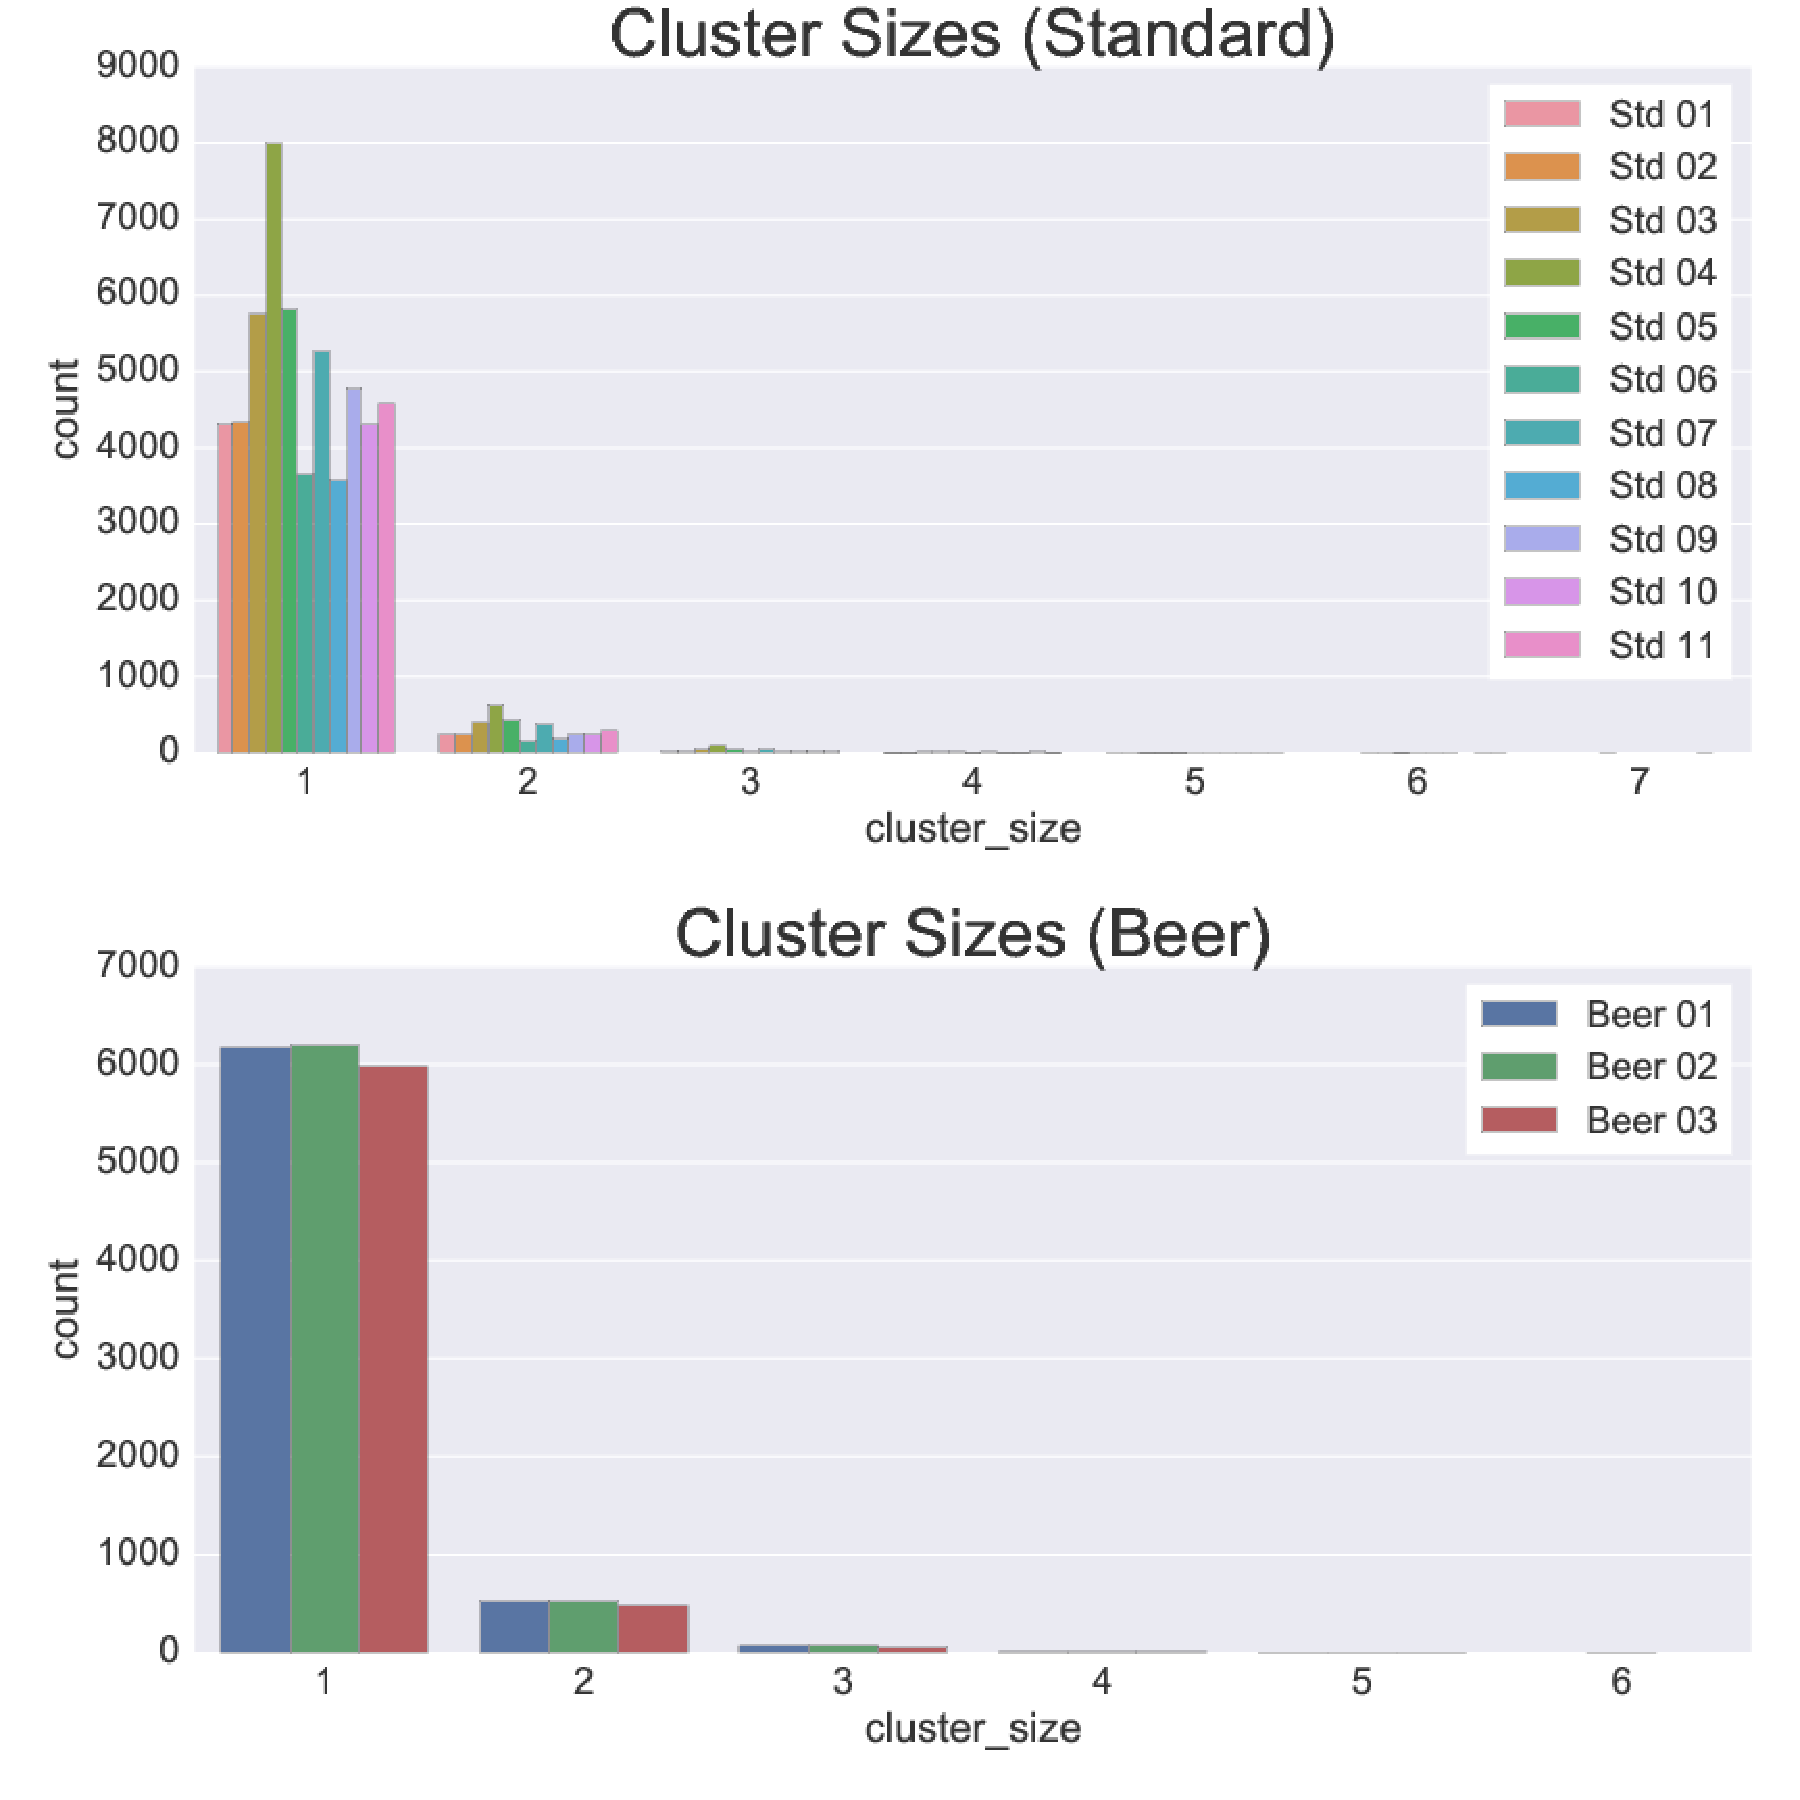
\includegraphics[width=0.5\linewidth]{05-precursor-cluster/figures/counts_cluster.pdf}
\caption{\label{fig:cluster-counts} Ionization product cluster sizes for all runs in the Standard and Beer datasets. For any given size, the number of clusters are generally more consistent in the Beer runs compared to the Standard runs, which shows greater variability due to the differences in the number of peak features per run.}
\end{figure}

Consistent with the number of singleton clusters, the M+H transformation dominate in the data. Non M+H transformations comprise 8\% of the total MAP transformations for the Standard dataset and 10\% for the Beer dataset. In both datasets, the M+ACN+H and M+Na transformations are highly prevalent (Figure~\ref{fig:counts-trans}). The presence of the M+ACN+H and M+NH4 transformations in the Beer dataset is expected, given the use of acetonitrile and ammonium carbonate buffers during chromatography. Similarly, the M+CH3OH+H adducts in the Beer data can also be explained by the use of methanol during the sample preparation process. The consistency of the example clusters in Figure~\ref{fig:06} and the explainable transformations in Figure~\ref{fig:counts-trans} suggest a valid result from PrecursorCluster, providing confidence that it can be used for alignment. 

\begin{figure}[htbp]
\centering
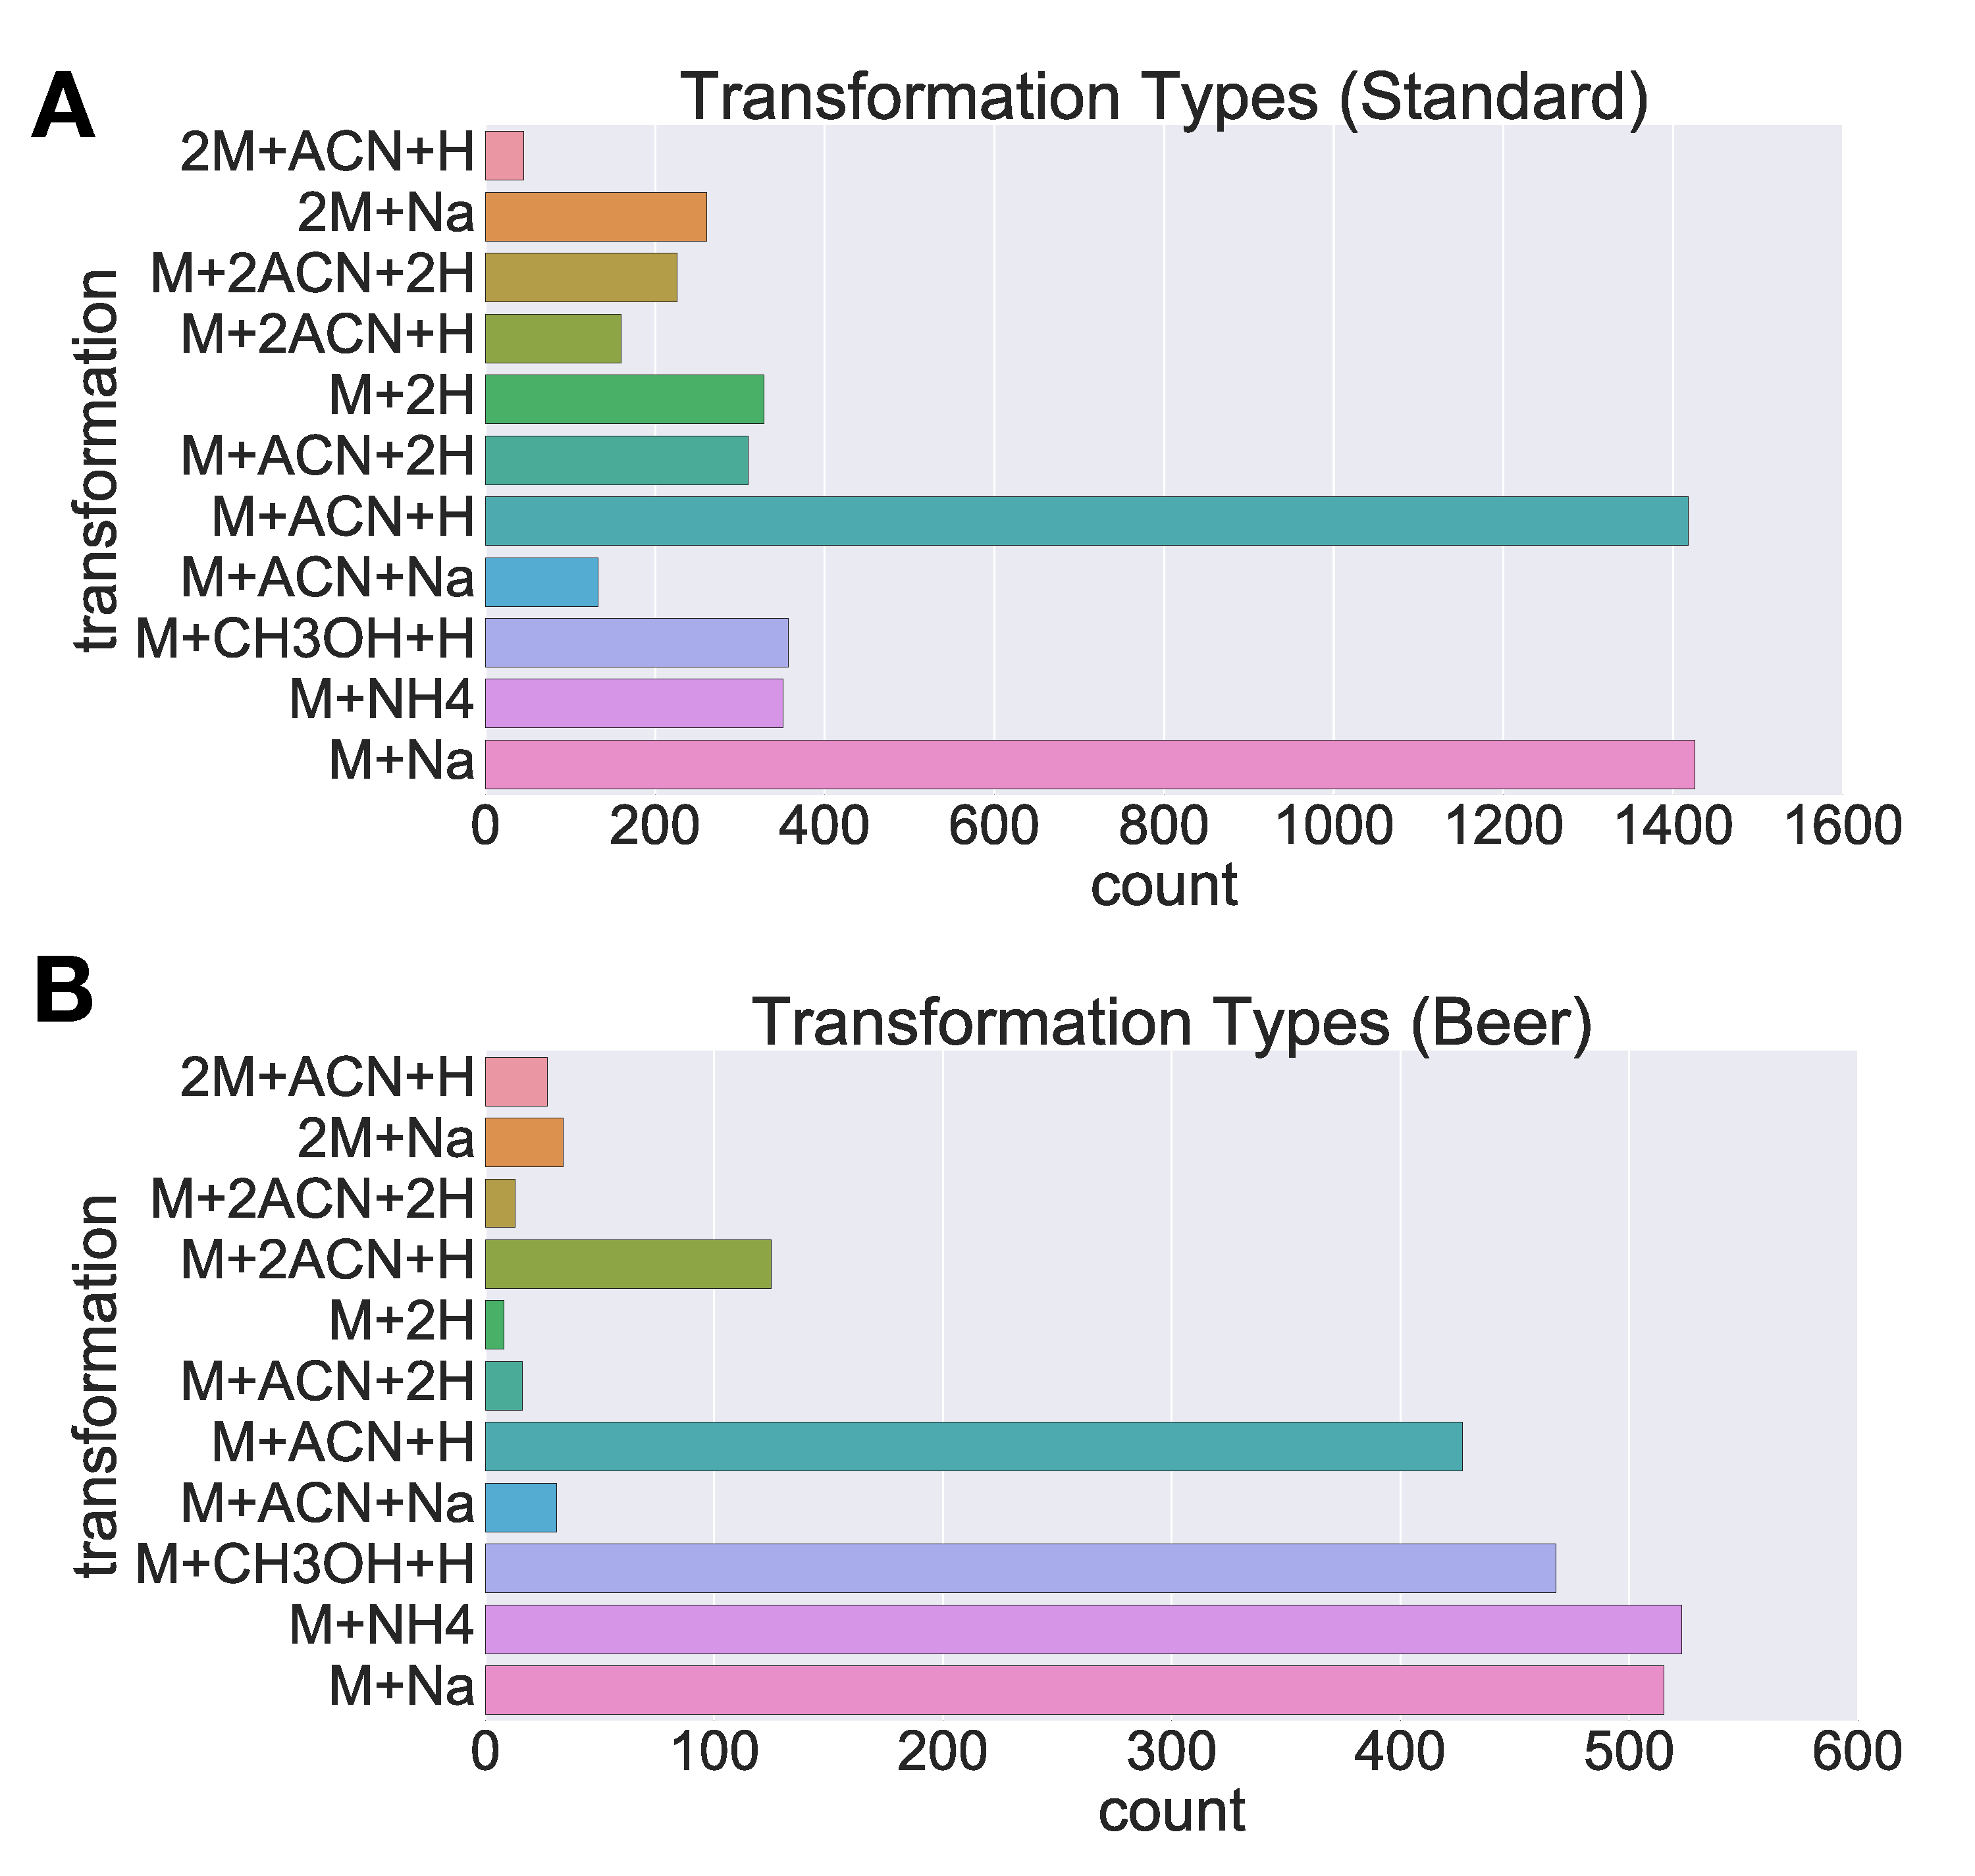
\includegraphics[width=0.5\linewidth]{05-precursor-cluster/figures/transformation_counts.pdf}
\caption{\label{fig:counts-trans}Barcharts showing the counts of transformation types in all Standard and Beer runs, excluding the M+H transformation.}
\end{figure}

\subsection{Improved Alignment Performance from Cluster-Match\label{sub:cluster-match-results}}

Precision and recall values produced by the different methods (across all parameter ranges) for the entire 30 Standard training sets and the 3 Beer runs can be found in Figure~\ref{fig:training-results}. Here, $l$ (the size of peakset combinations to be considered during performance evaluation) to 2 to consider only pairwise features for performance evaluation as pairwise performance limits overall performance in direct matching methods that employ the merge-match scheme to construct an overall result. The results in Figure~\ref{fig:training-results} (top row) shows that across all the m/z and RT window tolerances varied, Cluster-Match can produce higher precision while retaining similar recall values to feature matching (MW) or modified feature matching (MWG). This increase in precision comes from the increase of true positives and the decrease in false positives by taking into account the ionization product relationships between peak features when constructing the matching. The results here suggest that, regardless of the parameters selected for the m/z and RT tolerance windows, the proposed methods of matching by IP clusters can return a better alignment result compared to matching by peak features only.

Similar results can also be observed for the Beer dataset (Figure~\ref{fig:training-results}, bottom row). The complex Beer runs being aligned have minimal RT deviations when compared to the Standard runs, so all evaluated methods perform well, demonstrating smaller deviations in performance values despite varying the tolerances parameters. Again a general increase in precision of the results from Cluster-Match is observed over the other two baseline methods. MWG, which relies on the grouping of related peaks using their retention time values only, does not appear to produce any improvements over MW. The results here suggest that on complex LC-MS data such as the Beer data, the richer information present in the m/z and RT values of related peak features, alongside their possible IP transformations and relationships to the precursor peak, is essential and has to be taken into account.

\begin{figure*}[!htbp]
\centering
\centering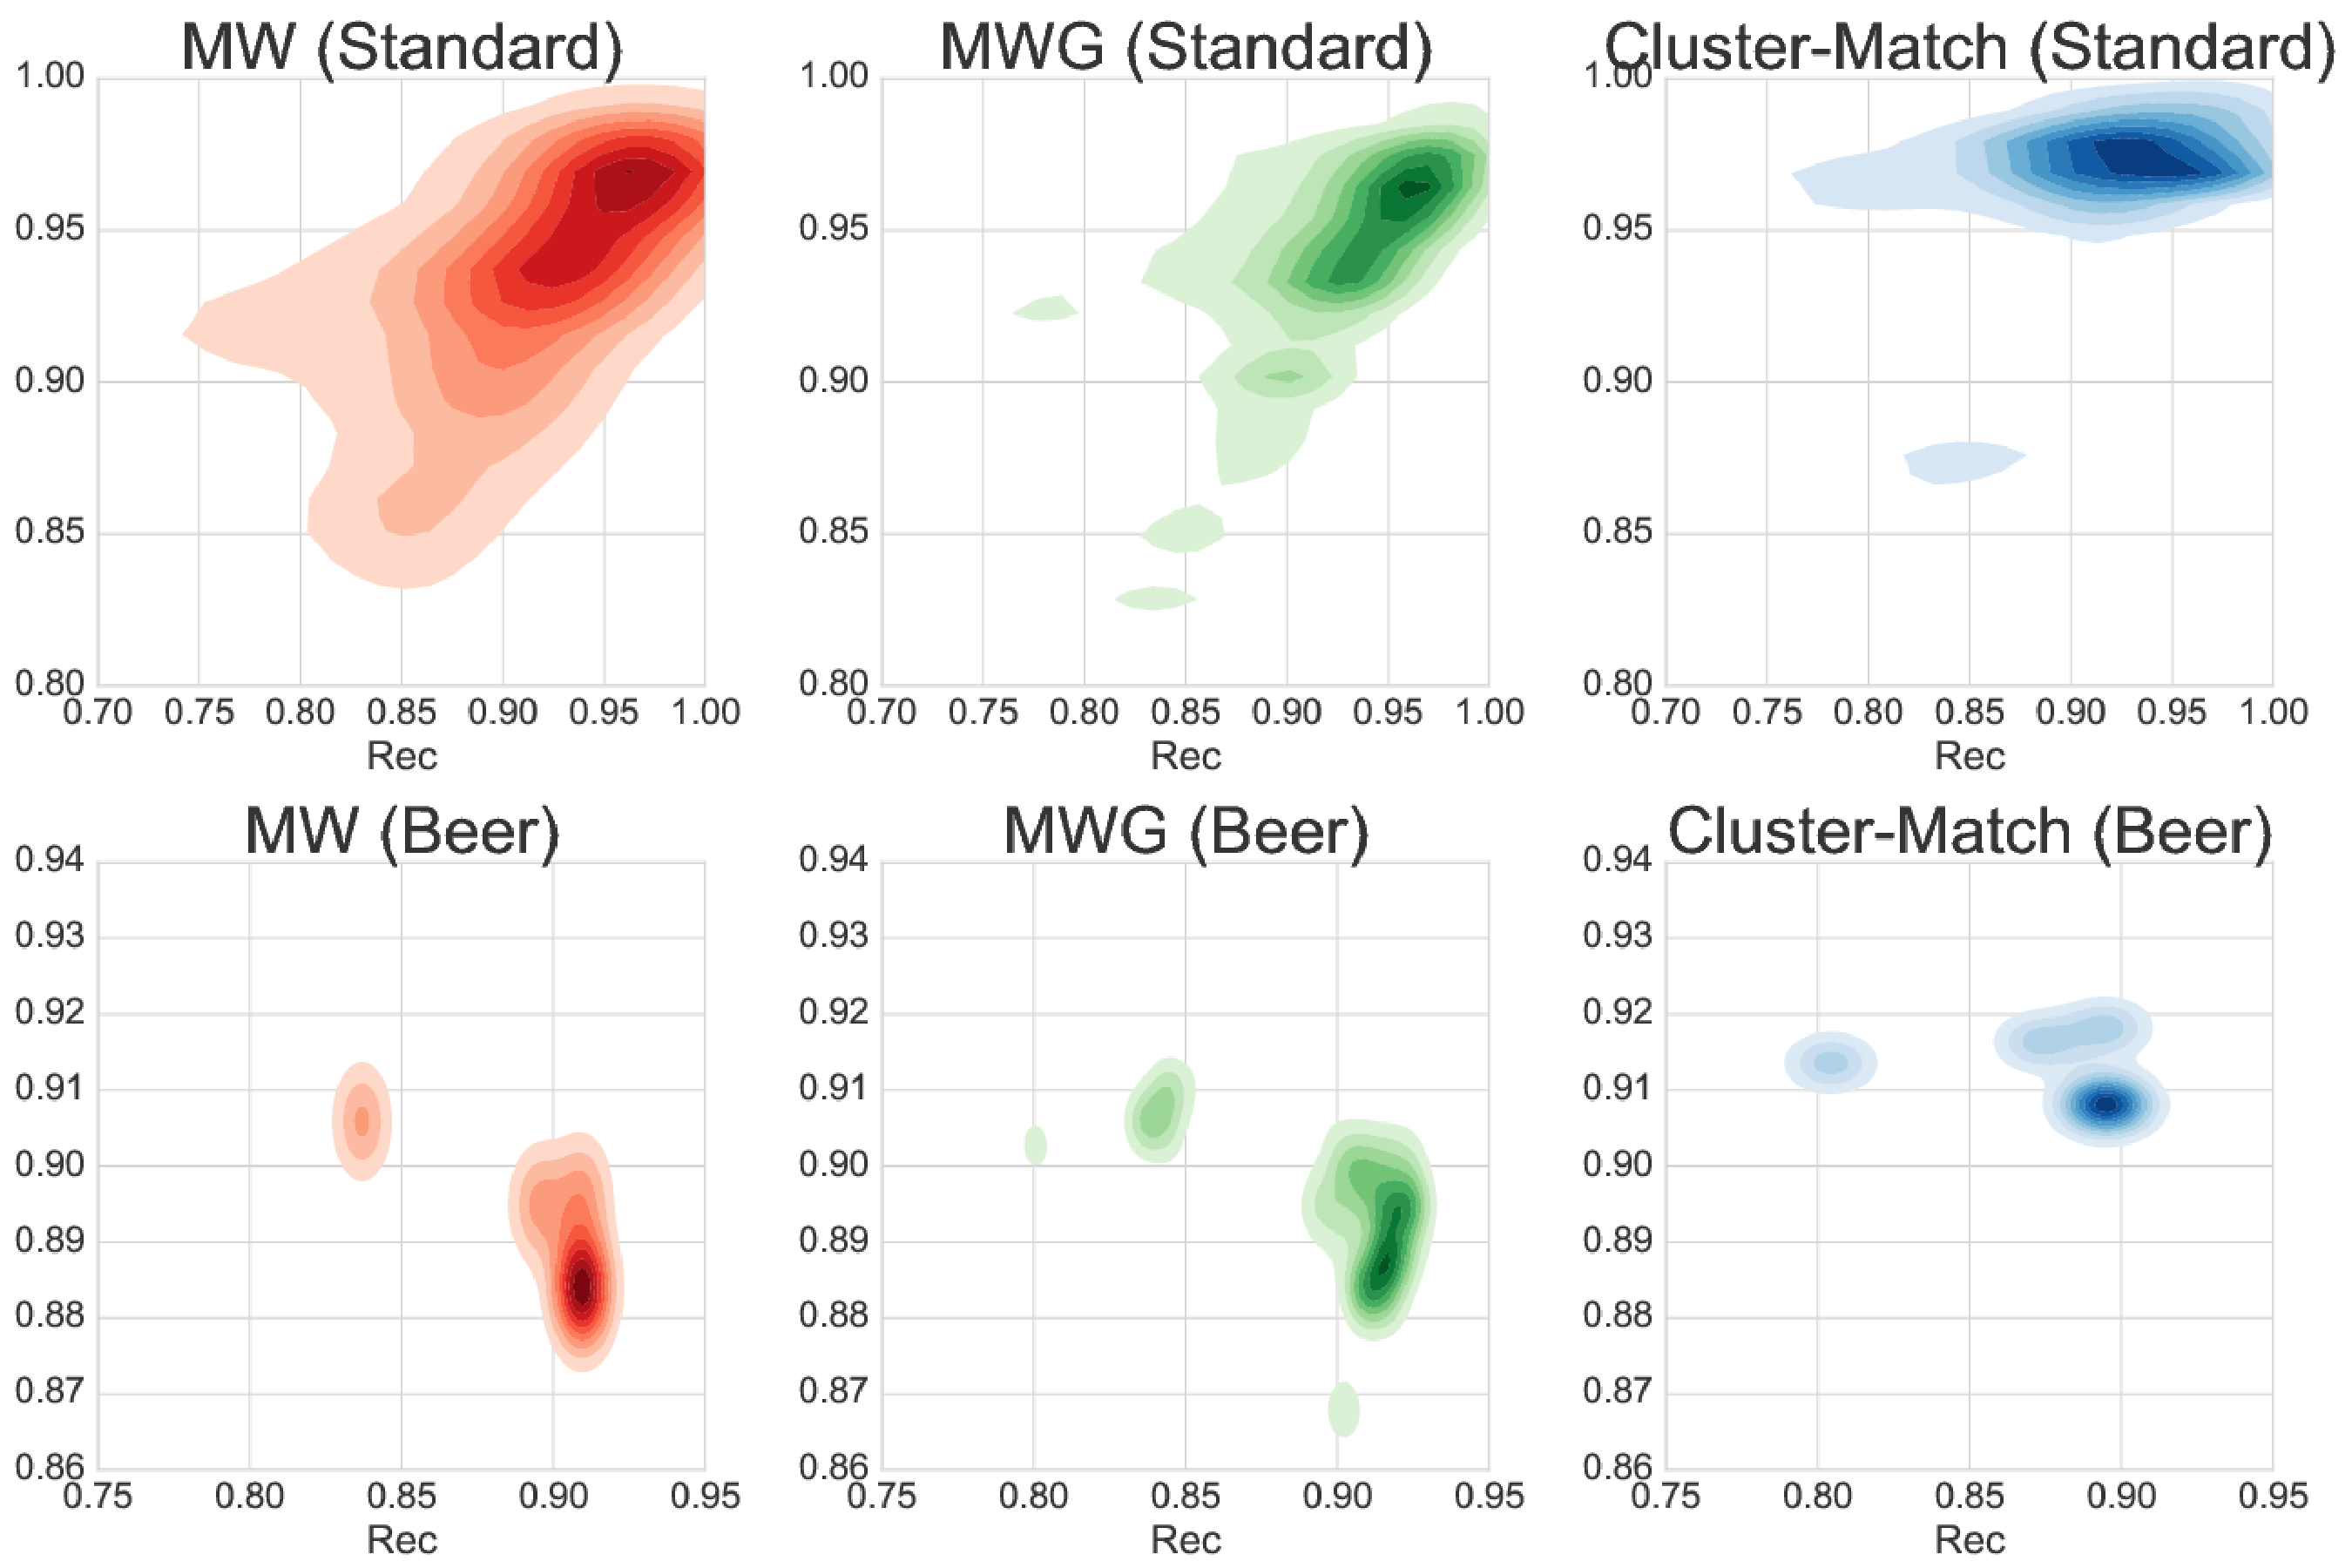
\includegraphics[width=1.0\linewidth]{05-precursor-cluster/figures/fig2.pdf}
\caption{\label{fig:training-results} All the training results obtained by varying the m/z and RT window parameters from the alignment of the entire 30 sets of pairwise Standard runs (top row) and the 3 Beer runs (bottom row). For MWG, the grouping parameter $t$ and score contribution $\alpha$ were also varied, while for Cluster-Match, the same set parameters of first-stage clustering was used for all input files.}
\end{figure*}

Optimizing parameters on the training set and evaluating performance on the testing set measures how well a method generalizes to new and unseen data. The best Standard training and testing $F_1$-scores from each method are reported in Figure~\ref{fig:pairwise-training-testing}. Using a one-sided paired t-test, Cluster-Match is found to be statistically greater than that of MW in both the training (p-value=0.002) and the testing cases (p-value=0.026), suggesting that Cluster-Match generalizes better to new and unseen datasets. MWG produces even higher training $F_1$-scores compared to the other two methods. This difference is found to be statistically significant using a one-sided paired t-test (p-value=0.01). The higher training performance of MWG can be explained by the fact that the RT grouping tolerance parameter and matching ratio for MWG were optimized during the training phase, while the same (potentially non-optimal) clustering parameters were used for the ionization product clustering of all Standard runs. On the testing results, no statistically significant differences were found on the testing $F_1$-scores of MWG and Cluster-Match, suggesting that both methods generalize well. 

\begin{figure}[!htbp]
\centering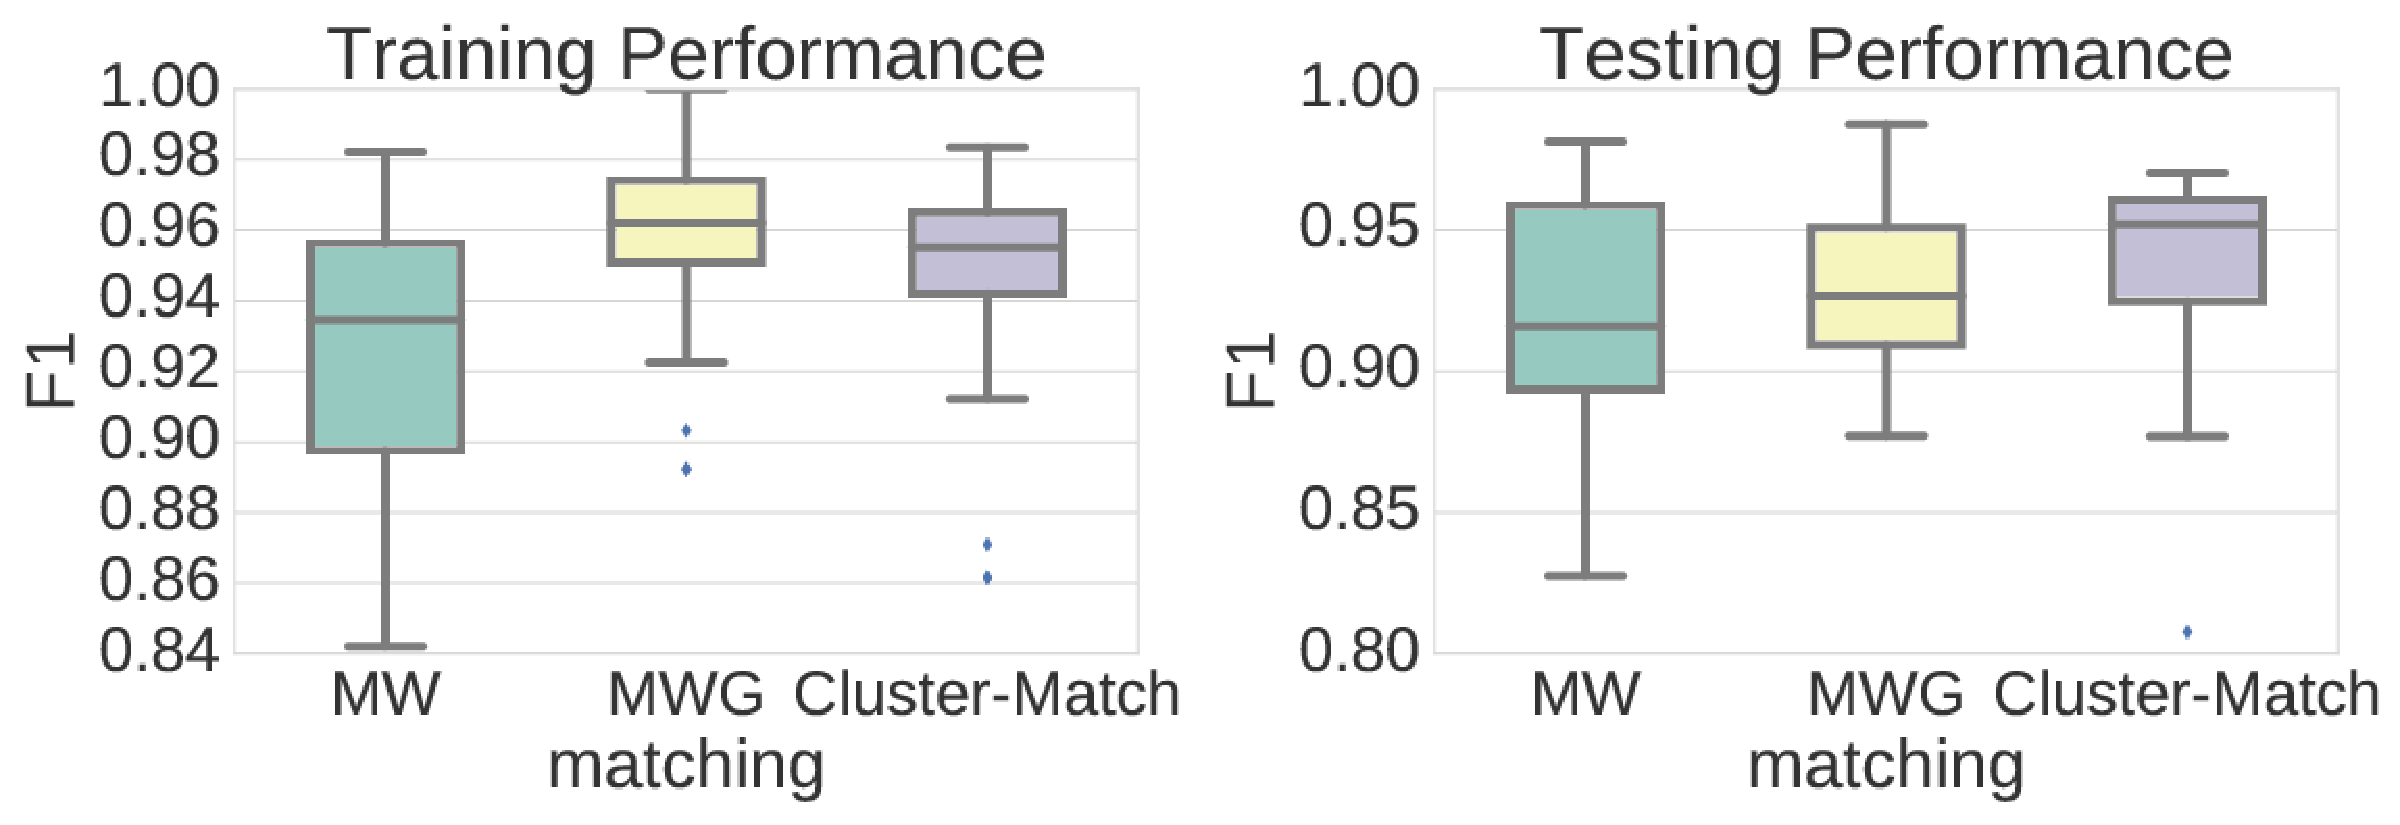
\includegraphics[width=0.75\linewidth]{05-precursor-cluster/figures/fig3.pdf}
\caption{\label{fig:pairwise-training-testing} The best training and testing $F_1$-scores obtained from the alignment of 30 sets of pairwise Standard runs.}
\end{figure}

\subsection{Probabilistic Matching Results from Cluster-Cluster\label{sub:cluster-cluster-results}}

Direct-matching methods such as MW and Cluster-Match can only return a definite matching solution to the alignment problem (a peak from one run is either aligned to a peak in the other run, or not). In contrast, the second-stage clustering process of the IP clusters employed in the Cluster-Cluster method allows us to produce an estimate in the uncertainties of matching of peak features, producing as the alignment result a list of aligned peaksets that have been matched at varying levels of confidence. Figure~\ref{fig:pr-curve} shows how a Precision-Recall (PR) curve, which shows how precision and recall change together, can be computed from the output of Cluster-Cluster on one of the sets of 4 randomly selected Standard runs and the set of 3 Beer runs. In Figure~\ref{fig:pr-curve}, the PR curves are plotted alongside the results from Cluster-Match at varying m/z and RT tolerance parameters (note that for Cluster-Cluster, we used only one set of potentially sub-optimal parameters for the second-stage clustering). Along both the PR curves on Figure~\ref{fig:pr-curve}, we see that generally, a decrease in the recall values is accompanied by an increase in the precision values. This applies to both the Standard and the Beer datasets, suggesting that by setting an appropriate threshold on the probabilities of aligned peaksets returned by Cluster-Cluster, we can obtain fewer aligned peaksets (lower recall) but at a higher confidence level of being correctly aligned (higher precision). In the face of further uncertainties with regard of user-defined parameters from the previous parts of the pipeline, the probabilistic alignment results returned by Cluster-Cluster allows the user to focus on peaksets of high matching confidence for subsequent analysis.  This introduces the possibility of returning a smaller subset from the overall aligned peaksets that have a higher confidence score of being correctly aligned --- an ability that few other matching methods can provide.

\begin{figure}[!htbp]
\centering
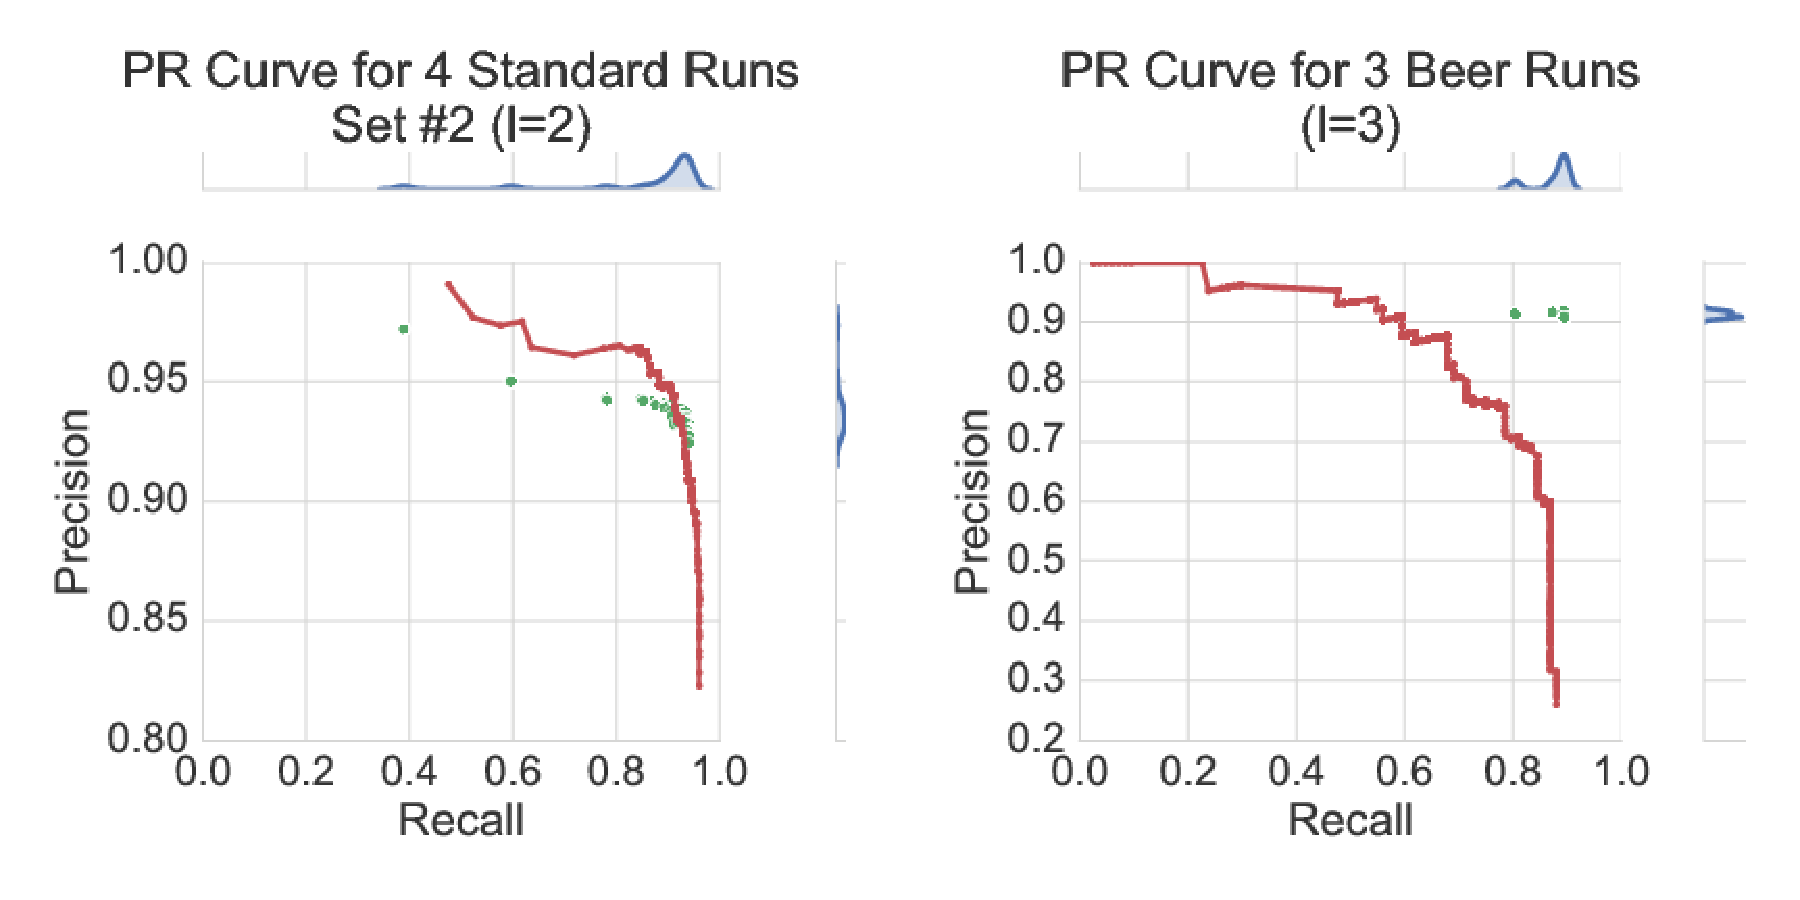
\includegraphics[width=1.0\linewidth]{05-precursor-cluster/figures/fig4.pdf}
\caption{\label{fig:pr-curve} PR curves obtained from running Cluster-Cluster on one of the sets of 4 randomly selected Standard runs (left) and the 3 Beer runs (right). Green dots are performance points obtained from running Cluster-Match at varying m/z and RT tolerance parameters on the same datasets, with their distributions of the points plotted along the marginals. The same first-stage clustering results were used as input to both Cluster-Match and Cluster-Cluster.}
\end{figure}

The results in Table~\ref{Tab:standard-beer-results} from running Cluster-Cluster, averaging over the sets of 2, 3, and 4 Standard runs, and on the entire 3 Beer runs, demonstrate that by setting some threshold values $\{0.30, 0.60, 0.90\}$ on the aligned peakset probabilities, various precision and recall values can be extracted. Upon aligning the sets of 4 Standard runs at threshold=0.30, Cluster-Cluster has a lower average precision of 0.81 than the best average performance from Cluster-Match at precision=0.87. Raising the threshold to 0.90 (consequently, decreasing recall as fewer aligned peaksets are returned) produces an average precision=0.90 for Cluster-Cluster, higher than 0.87 for Cluster-Match. On the complex Beer data, Cluster-Cluster produces precision=0.76 at threshold 0.30. Increasing the threshold to 0.90 produces a precision=0.94, which is again higher than the best attainable precision=0.91 from Cluster-Match. This demonstrates how recall can be traded for precision in Cluster-Cluster; a potentially useful ability in untargeted metabolomics experiments when the alignment ground truth is not available. In this situation, analysis effort can be focused on aligned peaksets with high confidence. 

The importance of the adduct fingerprint term is shown in Table~\ref{Tab:standard-beer-results}. Without the adduct fingerprint, a significantly lower $F_1$-score is produced by Cluster-Cluster at the probability threshold 0.90 \textbf{have you done any statistical testing on the results?}. This can be explained by the fact that excluding the adduct fingerprint term allows IP clusters having highly similar precursor mass and RT values to be placed in the same top-level cluster, despite each having an entirely different set of member adduct ions (and potentially corresponding to different metabolites). More false positive alignment items are produced, resulting in lower recall and $F_1$ scores. Using Figure~\ref{fig:06} as an example, the aligned peakset consisting of the four $[M+H]^+$ peaks in Figure~\ref{fig:06} has a high matching probability (0.97) when the adduct fingerprint term is used and almost never be placed together (near 0 probability) without. Similar observations can be concluded for the ions for other transformation types (e.g. the $[M+Na]^+$, $[M+ACN+H]^+$ adduct ions, etc.) shared by the clusters in Figure~\ref{fig:06}. The inclusion of the adduct fingerprint term in Cluster-Cluster is necessary to ensure that well-calibrated probabilities on the alignment results are obtained, especially on aligned peaksets with higher matching confidence.

\begin{table}[htbp]
\centering
\caption{Precision, recall and $F_{1}$ values from Cluster-Cluster for randomly selected sets of 2, 3 and 4 Standard runs (averaged) and the Beer runs for various $l$ and thresholding levels $th=\{0.30, 0.60, 0.90\}$. Best results from Cluster-Match and the result of running Cluster-Cluster without the adduct fingerprint term are shown for comparison. Note that for Cluster-Cluster, the results come from using one set of potentially sub-optimal parameters for the second-stage clustering.\label{Tab:standard-beer-results}}
\scalebox{0.75}{
\begin{tabular}{|l|c|c|c|c|c|c|c|c|p{2cm}|}
\hline 
\multirow{2}{*}{Dataset} & \multirow{2}{*}{$l$} & \multicolumn{3}{c|}{Best Cluster-Match} & \multicolumn{4}{c|}{Cluster-Cluster (CC)} & CC (without adduct term)\tabularnewline
\cline{3-10} 
 &  & Avg. Prec. & Avg. Rec. & Avg. $F_{1}$ & Threshold & Avg. Prec. & Avg. Rec & Avg. $F_{1}$ & Avg. $F_{1}$\tabularnewline
\hline 
\hline 
\multirow{3}{*}{Standard} & \multirow{3}{*}{2} & \multirow{3}{*}{0.93} & \multirow{3}{*}{0.92} & \multirow{3}{*}{\textbf{0.93}} & 0.30 & 0.96 & 0.95 & 0.95 & \textbf{0.95}\tabularnewline
\cline{6-10} 
 &  &  &  &  & 0.60 & 0.98 & 0.93 & \textbf{0.96} & 0.93\tabularnewline
\cline{6-10} 
 &  &  &  &  & 0.90 & 1.00 & 0.90 & 0.94 & 0.80\tabularnewline
\hline 
\multirow{3}{*}{Standard} & \multirow{3}{*}{3} & \multirow{3}{*}{0.89} & \multirow{3}{*}{0.90} & \multirow{3}{*}{\textbf{0.89}} & 0.30 & 0.82 & 0.91 & 0.84 & \textbf{0.86}\tabularnewline
\cline{6-10} 
 &  &  &  &  & 0.60 & 0.86 & 0.88 & \textbf{0.86} & 0.85\tabularnewline
\cline{6-10} 
 &  &  &  &  & 0.90 & 0.89 & 0.81 & 0.84 & 0.62\tabularnewline
\hline 
\multirow{3}{*}{Standard} & \multirow{3}{*}{4} & \multirow{3}{*}{0.87} & \multirow{3}{*}{0.92} & \multirow{3}{*}{\textbf{0.89}} & 0.30 & 0.81 & 0.92 & 0.85 & \textbf{0.89}\tabularnewline
\cline{6-10} 
 &  &  &  &  & 0.60 & 0.84 & 0.89 & 0.85 & 0.86\tabularnewline
\cline{6-10} 
 &  &  &  &  & 0.90 & 0.90 & 0.83 & \textbf{0.86} & 0.65\tabularnewline
\hline 
\multirow{3}{*}{Beer 3 runs} & \multirow{3}{*}{3} & \multirow{3}{*}{0.92} & \multirow{3}{*}{0.89} & \multirow{3}{*}{\textbf{0.91}} & 0.30 & 0.76 & 0.77 & \textbf{0.77} & \textbf{0.79}\tabularnewline
\cline{6-10} 
 &  &  &  &  & 0.60 & 0.88 & 0.67 & 0.76 & 0.68\tabularnewline
\cline{6-10} 
 &  &  &  &  & 0.90 & 0.94 & 0.54 & 0.68 & 0.63\tabularnewline
\hline 
\end{tabular}
}
\end{table}

\subsection{Running time}

Efficient inference is possible in PrecursorCluster as many peaks can only be placed in one cluster and need not be reassigned during Gibbs sampling. For the Standard runs with up to 5000 peak features, less than a quarter of peak features have to be reassigned. Taking 10000 posterior samples, Gibbs sampling for PrecursorCluster requires ~20 minutes to process one Standard run on an Intel Core i5, 3.3GHz PC. Runs are processed independently and can be parallelized. In Cluster-Match, the matching of IP clusters via MW has a time complexity of $O(m\, log\, n)$ time, where $n$ and $m$ are the number of vertices and edges in the bipartite graph to be solved, translating to a wall clock of less than a minute for each run. Cluster-Cluster requires longer computational time. With 1000 posterior samples per top-level bin, the processing of 2 Standard runs requires approximately half an hour. Each top-level bin can also be processed in parallel.

\section{Conclusions}

\textbf{Can you broaden this out a bit? It reads like a paper conclusion. You have no space limitation}

We have proposed an integrative workflow that performs the precursor clustering of ionization product peaks and uses that to improve alignment. The PrecursorCluster model introduced is a data reduction process that can reduce the number of objects to be aligned based on a list of possible ionization transformation types. The clustering information extracted from PrecursorCluster can be used to improve other steps in the pipeline too. For instance, metabolite identification, currently the main bottlenecks in high-throughput metabolomics, might be improved through analyzing IP clusters as the objects of interest rather than individual peak features. 

Through Cluster-Match, we have also demonstrated that IP clustering can be used to improve alignment, producing results that outperform the direct-matching of peak features alone. The proposed pairwise matching scheme used by Cluster-Match is frequently extended to the processing of multiple runs in a fairly ad-hoc manner and suffers from having to set a reference run (which can be considered another parameter to set). Producing a distance measure that works well for measuring similarities of peaks across multiple runs is non-trivial, and most methods do not take into account the uncertainties inherent in the matching of peak features across runs. Cluster-Cluster addresses these issues by not requiring a reference run and being able to return aligned peaksets at varying probabilities. As future work, PrecursorCluster can be improved by considering chromatographic shapes rather than RT values. An interactive visualisation module can be developed to let user visualize ionization product clustering and aligned peaksets (with their probabilities) from a single graphical interface. Such module can be incorporated as part of a larger metabolomics pipeline.

A weakness of the alignment methods described in this chapter is the fact that as a second-stage clustering step, both Cluster-Match and Cluster-Cluster requires the MAP assignment of peak features into their IP clusters. This means uncertainties in the ionization product clustering stage are not propagated to the matching stage. The next chapter addresses this problem by introducing a fully-hierarchical model that performs the clustering of peak features within run and across runs at once.